\documentclass[a4paper,18pt]{report}
\usepackage[top=2.5cm, right=2.0cm, left=2.0cm, bottom=3.0cm]{geometry}
\usepackage{graphicx}
\usepackage{subfigure}
\usepackage{amsmath}
\usepackage{algorithmic}
\usepackage{algorithm}
% Title Page
\title{Modelling the epidemiological and evolutionary dynamics of influenza outbreaks}
\author{Gayle Leen}


\begin{document}
\maketitle

\begin{abstract}

\end{abstract}

\section{Background}



\section{Notation}
\begin{itemize}
\item Number of hosts: $N_h$
\item $N_h$ sets of genetic sequences: $\mathcal{D} = \{\mathbf{D}_1,...,\mathbf{D}_{N_h}\}$, where $\mathbf{D}_i = \{\mathbf{d}_{i,1},...,\mathbf{d}_{i,P_i}\}$ ($P_i$ the number of sequences in host $i$)
\item Times of sampling the genetic sequences for each host: $\mathcal{S} = \{s_1,...,s_{N_h}\}$
\end{itemize}

\section{Overview}
This report describes a model of intrahost and between-host viral dynamics in an outbreak. Given a set of hosts, and within-host viral populations sampled from each infected host as the virus spreads throughout the population, the model infers transmission and evolutionary parameters                                                                   
that explain the pattern and timing of mutations in the hosts.

Each host is modelled as a population of $N$ `particles'. Initially susceptible to infection, I assume that this within-host population evolves according to SIR (susceptible, infected, recovered) dynamics. The evolution of the population of infected particles represents the dynamics of the virus in the host. I assume that this process is observed at the timepoints when a subset of the infected population is sampled from each host, resulting in the genetic sequences $\{\mathbf{D}_1,...,\mathbf{D}_{N_h}\}$. As well as representing the amount of virus in each host over time, the evolution of the infected particles gives rise to a genealogy underlying the infected population - when an infection event occurs (S $\rightarrow$ I), this corresponds to an infected particle giving birth to another (branching/birth event),
and a recovery event (I $\rightarrow$ R) corresponds to the death of an infected particle. This is similar to a birth death tree, where the birth and death rates vary according to the size of the current S and I populations.

Crucially, I allow infected particles to infect susceptible particles in other hosts, as well as within-host, to model the spread of the virus between hosts in a population. A simulation of the process produces a possible genealogy between all of the observed genetic sequences.

Finally, a mutation model is used to simulate the evolution of mutations along the genealogical tree, to generate the genetic sequence at each tip.

\section{Detailed overview of forward simulation} 

\begin{figure}[h]
\centering
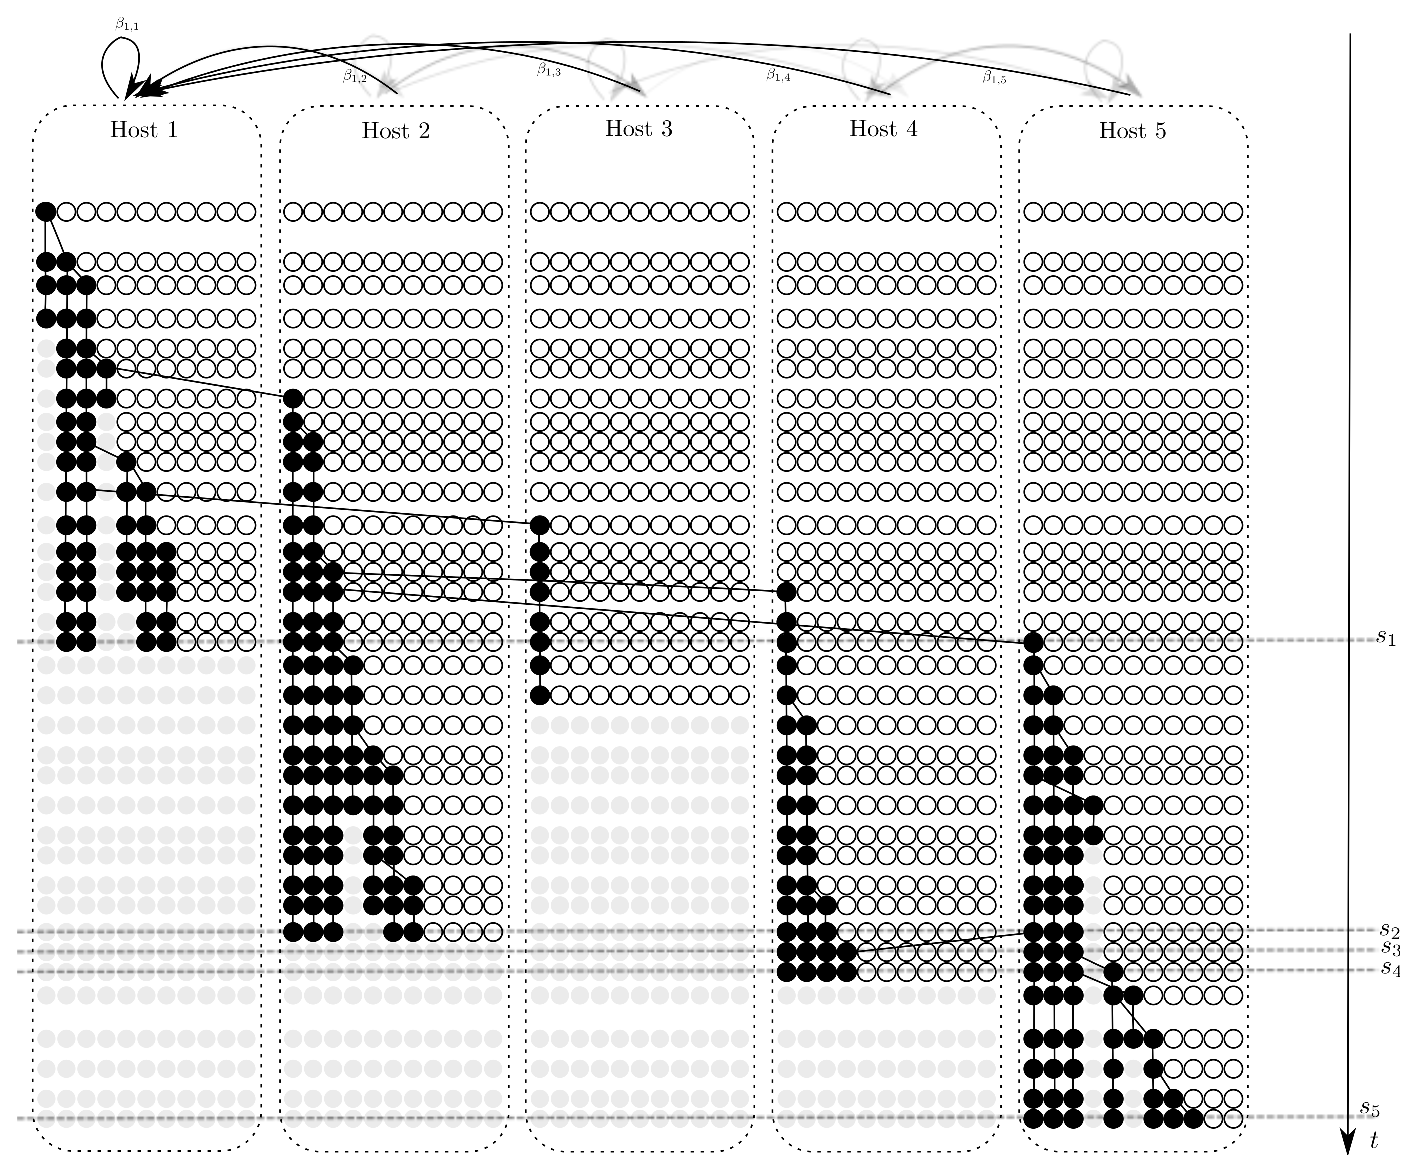
\includegraphics[width=0.8\textwidth]{model_1.eps}
\caption{Generation of genealogy for intrahost populations for $5$ hosts, observed at times $s_1$,...,$s_5$. Each host contains $N=11$ particles, which can be susceptible (white), infected (black), or recovered (grey). Initially (first row) all the particles are susceptible, except for $1$ infected in host $1$. The particles evolve according to the stochastic SIR process detailed in (\ref{eq:sirprocess}). Each infection is a birth event where the parent is chosen at random, and a recovery event is a death event for a randomly chosen infected particle.
}\end{figure}
Given the set of genetic sequences $\mathcal{D} = \{\mathbf{D}_1,...,\mathbf{D}_{N_h}\}$, observed at times $\mathbf{S} = \{s_1,...,s_{N_h}\}$ respectively, denote the underlying genealogy as $\mathcal{G}$. 
For a given $\mathcal{G}$, and mutation model, we can calculate the probability of $\mathcal{D}$ as shown in the next section. 
\subsection{Mutation model}
Associated with each leaf node of $\mathcal{G}$ is a nucleotide sequence (denote a sequence as $d_{h,i}$ ($h$ = host, $i$=sequence number in $h$'s viral population) . A likelihood can be calculated for the sequences at the tips of the tree ; we use the standard finite-sites selection-neutral likelihood framework with a general time-reversible (GTR) substitution model. Suppose that each of the sequences has length $L$, and at each site $l$ each base character in the sequence can take on values in the set $\mathcal{C}=\{A,C,G,T\}$. We use a mutation model that assumes that each site mutates in forward time according to a Poisson jump process, parameterised by a ($4 \times 4$) rate matrix $\mathbf{Q}$ where $\mathbf{Q}_{ij}$ is the instantaneous rate for the transition from character $i$ to character $j$ (A=$1$, C=$2$, G=$3$, T=$4$). The time units of the rates in $\mathbf{Q}$ are chosen such that the mean number of mutations per unit time occurring at a site is equal to $1$, and we scale this with parameter $\mu$, which represents the mean number of mutations per calendar unit at a site. 
To derive the likelihood, we consider an edge between parent $i$ and child $j$, $e_{ij}$ in $\mathcal{G}$. $j$ is a direct descendant of $i$, but the sequences $D_i$ and $D_j$ may be different if a mutation has occurred along the branch between $i$ and $j$. In this framework, the probability of a character at site $l$ in child $j$, given parent $i$, is expressed as $P(D_{j,l} = c' | D_{i,l} = c)=[\exp(-\mathbf{Q}\mu|e_{ij}|)]_{c,c'}$, for $c,c' \in \mathcal{C}$, and $|e_{ij}|$ is the edge length between $i$ and $j$. 

Let $\mathcal{D}$ denote the set of sequences associated with the tree tips, and $\mathcal{D}_A$ denote the (unknown) sequences associated with the ancestral / interior nodes. The probability for any particular set of sequences $\{\mathcal{D}, \mathcal{D}_A\}$ to be realised at the nodes of tree $\mathcal{G}$ is given by:
\begin{eqnarray}
P(\{\mathcal{D}, \mathcal{D}_A\}\mid \mathcal{G},\mu)=\prod_{\{i,j\}\in e} \prod_{l=1}^L [\exp(-\mathbf{Q}\mu|e_{ij}|)]_{D_{i,l},D_{j,l}}\label{eq:mut1}
\end{eqnarray}
We can integrate over the unknown $\mathcal{D}_A$ by summing over all sets of possible ancestral sequences $\mathbf{D}_A$.
\begin{eqnarray}
P(\mathcal{D}\mid \mathcal{G},\mu)=\sum_{\mathcal{D}_A \in \mathbf{D}_A} P(\{\mathcal{D}, \mathcal{D}_A\}\mid \mathcal{G},\mu)\label{eq:mut2}
\end{eqnarray}
which can be evaluated using a pruning algorithm \cite{felsenstein:1981}. 

\subsection{Population history model}
A genealogy $\mathcal{G}$ which gives rise to $\mathcal{D}$ will have $\sum_i P_i$ tips (the number of sequences), where each host's set of tips end at the corresponding sampling times $s_1,...,s_{N_h}$. Since a bifurcating tree is assumed, there are $(\sum_i P_i)-1$ interior nodes, which bifurcate at unknown times $\mathbf{b}=\{b_1,...,b_{(\sum_i P_i)-1}\}$. The genealogy can be completely specified by the bifurcation times, and the topology $\mathcal{T}$ ; $\mathcal{G}=\{\mathbf{b}, \mathcal{T}\}$. 

The bifurcation times of the genealogy depend on the population dynamics of the particles / viruses which are sampled. For instance,  suppose that the mutation rate is high and we compare the sequences of a pair of viruses from the population at a time point: the pair of sequences are likely to be less similar if the population size is large, and vice versa - i.e. for a large population size, a common ancestor of two sequences would be further back in time, and the genealogy would have longer branch lengths. In our model, we use a stochastic model of viral population dynamics to model the growth of the infected population in each host, allowing transmission between each intrahost population.
\subsubsection{Intrahost population trajectories}
For host $h$, we model the intrahost viral population as following SIR (susceptible, infected, recovered) dynamics. Let $S_h(t), I_h(t)$ and $R_h(t)$ denote random variables for the 
number of susceptible, infected, and immune `particles' respectively, where $S_h(t) + I_h(t) + R_h(t) = N$, where $N$ is the size of the viral population. We assume the following transition probabilities:
\begin{eqnarray}
P(\Delta S_h(t) &=& i, \Delta I_h(t) = j \mid S_1(t), I_1(t),..., S_{N_h}(t), I_{N_h}(t)) \label{eq:sirprocess}\\
&=& \left\{\begin{tabular}{l l l}
$\frac{\beta_{h,h'}}{N}S_h(t)I_{h'}(t)\Delta t + o(\Delta t)$, \hspace{0.4cm} & $h= h' : (i,j)=(-1,1)$ &  \\ 
& $h \neq h' : (i,j)=(-k_{h'}(t),k_{h'}(t))$ & \\
$\gamma I_h(t) \Delta t + o(\Delta t)$, & $(i,j)=(0,-1)$ & \nonumber\\
$1 - (\sum_k \frac{\beta_{h,k}}{N}S_h(t)I_k(t)\Delta t $ &  &\\
$+ \gamma I_h(t) \Delta t) + o(\Delta t)$, & $(i,j)=(0,0)$ &
\end{tabular}\right.
\end{eqnarray}
where $k_h$ is the number of particles that is transmitted from host $h$. We generate $k_h$ from a Binomial distribution $\textrm{Bin}(N, \phi_K)$

We generate the intrahost population trajectories via the Gillespie algorithm. There are $N_h(N_h+1)$ possible events:
$N_h \times N_h$ birth / infection events, and  $N_h$ death / recovery events. Denote their rates by $N_h \times (N_h+1)$ matrix $\mathbf{E}(t)$,
where $\mathbf{E}_{i,j}(t)=\frac{\beta_{i,j}}{N}S_i(t)I_j(t)$ is the rate at which host $j$ infects host $i$, and $\mathbf{E}_{i,N_h+1} = \gamma I_i(t)$ is the death rate in host $i$.

We keep track of the events in a matrix $\mathbf{T}$, where the $i$th row (corresponding to the $i$th event) is $\mathbf{T}_i=\{t_i, h_a, h_b, v\}$, where $t_i$ is the time of the event,
$v$ is the type of event $v \in \{-1,1\}$ (death, birth respectively) from host $h_b$ to $h_a$. See Algorithm \ref{alg:pts}.
\begin{algorithm}
\caption{Population trajectory sampling \label{alg:pts}}
\begin{algorithmic}
\STATE $t\gets 0$
\STATE $\mathbf{I}(0)\gets\{I_1(0)=1, I_2(0)=0, ..., I_{N_h}=0\}$
\STATE $\mathbf{S}(0)\gets\{S_1(0)=N-1, I_2(0)=N, ..., I_{N_h}=N\}$
\WHILE{$\sum_k I_k(t) > 0$}
\STATE Generate $k_h$
\STATE $t_e \sim \textrm{Exp}(\sum_k \frac{\beta_{h,k}}{N}S_h(t)I_k(t) + \gamma I_h(t))$ \COMMENT{Draw time until next event}
\STATE $e \sim \text{Categorical}(\mathbf{E}(t+t_e))$  \COMMENT{Draw event}
\STATE $t \gets t+t_e$
\STATE Update $\mathbf{I}(t), \mathbf{S}(t), \mathbf{T}$, based on $e$.
\ENDWHILE
\end{algorithmic}
\end{algorithm}

\subsubsection{Intrahost population trajectories given the data}

Given the sampling times $\{s_1,...,s_{N_h}\}$, and assuming that $P_h$ infected lineages in host $h$  are removed after sampling at time $s_h$, we modify the algorithm as shown in Algorithm \ref{alg:ptsd}.
\begin{algorithm}
\caption{Population trajectory sampling given data \label{alg:ptsd}}
\begin{algorithmic}
\STATE $t\gets 0$
\STATE $\mathbf{I}(0)\gets\{I_1(0)=1, I_2(0)=0, ..., I_{N_h}=0\}$
\STATE $\mathbf{S}(0)\gets\{S_1(0)=N-1, I_2(0)=N, ..., I_{N_h}=N\}$
\WHILE{$\sum_k I_k(t) > 0$}
\STATE Generate $k_h$
\STATE $t_e \sim \textrm{Exp}(\sum_k \frac{\beta_{h,k}}{N}S_h(t)I_k(t) + \gamma I_h(t))$ \COMMENT{Draw time until next event}
\FOR{$h=1$ to $N_h$}
{\IF{$t+t_e>s_h$} 
\STATE $I_h(t+t_e)\gets I_h(t+t_e) - P_h$ 
\STATE Update $\mathbf{T}$
\ENDIF}
\ENDFOR
\STATE $e \sim \textrm{Categorical}(\mathbf{E}(t+t_e))$  \COMMENT{Draw event after updating $\mathbf{E}$}
\STATE $t \gets t+t_e$
\STATE Update $\mathbf{I}(t), \mathbf{S}(t), \mathbf{T}$, based on $e$.
\ENDWHILE
\end{algorithmic}
\end{algorithm}
In order to simulate $\mathcal{G}$ which gives a non-zero likelihood $p(\mathcal{D}\mid \mathcal{G}, \mu)$, we require the number of infected particles in the hosts when they are observed at times $\mathbf{S}=\{s_1,...,s_{N_h}\}$ to be consistent with the data $\mathcal{D}$.  We write the prior for the set of infected population trajectories $\mathbf{I}(t)$ as:
\begin{eqnarray}
p(\mathbf{I}(t) \mid  \gamma, \{\beta_{1,1},...,\beta_{N_h,N_h}\}, N, \phi_K, t_{off})
\end{eqnarray}
which can be sampled via simulation by Algorithm \ref{alg:ptsd}, where $t_{off}$ denotes the time between the start of the trajectory and the first sampling time. Denoting $P_i$ as the number of sequences in host $i$, sampled at time $s_i$, we only accept the simulated trajectory if the number of surviving lineages (tips) at times $s_1,...,s_{N_h}$ in hosts $1,...,N_h$ are $\{ \geq P_1,..,\geq P_{N_h}\} $ respectively.
%The likelihood of $\mathcal{G} = \{\{b_1,...,b_{(\sum_i P_i)-1}\},\mathcal{T}\}$ under the data (the number of sequences and their time of sampling) is given by:
%\begin{eqnarray}
%p(P_1,...,P_{N_H} \mid \mathcal{G}, \mathbf{S}) \label{eq:113}
%\end{eqnarray}
%which will be $1$ if the number of surviving lineages (tips) at times $s_1,...,s_{N_h}$ in hosts $1,...,N_h$ are $\{ \geq P_1,..,\geq P_{N_h}\} $ respectively, and $0$ otherwise.
%To draw a sample from 
%\begin{eqnarray}
%p(\{\mathcal{G} \mid \gamma, \{\beta_{1,1},...,\beta_{N_h,N_h}\}, N, N_h, P_1,...,P_{N_H}, \mathbf{S}) \label{eq:ll2}
%\end{eqnarray}
%we draw $\mathcal{G}$ according to $I(t)$, from the SIR process, and accept the sample if (\ref{eq:ii3}=$1$).

\subsection{Reconstructed tree and bifurcation times}
We relate the infected population trajectory $\mathbf{I}(t)$ to a genealogical tree: each birth / infection event is a bifurcation event (a lineage splits in two), and recovery is the death of a lineage. Each lineage corresponds to an infected particle, and for each event, a particle is picked at random.
See Figure \ref{fig:tree1}. We then remove extinct lineages to get a 'reconstructed tree' (see Figure \ref{fig:tree2}). This results in a genealogy that underlies the set of observed sequences  $\mathbf{G}$, generated by a birth-death process, where the birth and death rates are governed by SIR dynamics (\ref{eq:sirprocess}), with  $\sum_i^{N_h} P_i - 1$ bifurcations / coalescent events at times $\mathbf{b}=\{b_1,...,b_{(\sum_i P_i)-1}\}$, and the topology $\mathcal{T}$ is partially defined on a host-host level, since we know which host each particle is in. Let's record the bifurcation times $\mathbf{b}$ and partial topology in matrix $\mathbf{T}^R$, where the $i$th row corresponds to the $i$th bifurcation event: $\mathbf{T}^R_i=\{b_i, H_p, H_{c_1}, H_{c,2}\}$, where $H_p, H_{c_1}, H_{c,2}$ are the hosts of the parent, and two children. We can generate the full topology from $\mathbf{T}_R$. Algorithm \ref{alg:g_from_I} describes how the genealogy can be constructed from a population trajectory $\mathbf{I}$. 

\begin{algorithm}
\caption{Reconstructing ancestral tree $g$ from infected population trajectories $I[t]$, $\mathbf{T}$ \label{alg:g_from_I}}
\begin{algorithmic}
\STATE ${\textrm{Nodes}_{\textrm{anc}}=\{\}}$ , ${\textrm{t}_{\textrm{anc}}=\{\}}$ \COMMENT{list of ancestral nodes and times, for each host}
\STATE ${\textrm{Nodes}_{\textrm{ex}}}=\{I[T][1] - P_1, ..., I[T][N_H] - P_{N_H}\}$,   \COMMENT{vector of number of extinct nodes for each host}
\STATE $g=\{\}$ \COMMENT{ancestral tree}
\STATE $n_{\textrm{int}}= N_s + 1$ \COMMENT{internal node of tree}
\STATE Label sequences in $\mathcal{D}$ for each host: $\mathcal{L}_1=\{1,...,P_1\}$,  $\mathcal{L}_2=\{P_1+1,...,P_1 + P_2\}$, 
\FOR{$t=T$ \TO $t=1$ \COMMENT{for each event time}}
{
\IF{$t=s_i$, where $i \in 1,...,N_H$ \COMMENT{if at sampling time for host i}}	
{
	\STATE $\textrm{Nodes}_{\textrm{anc}}[i] \gets \mathcal{L}_i $
	\STATE $\textrm{t}_{\textrm{anc}}[i] \gets \{t, t, ..., t\}$
}
\ENDIF
\IF{event at $t$ = recovery in host $i$}	
	\STATE $\textrm{Nodes}_{\textrm{ex}}[i] \gets \textrm{Nodes}_{\textrm{ex}}[i]  + 1 $
\ENDIF
\IF{event at $t$ = infection within host $i$}	
{
	\STATE Pick a pair of nodes $n_a$, $n_b$ from all nodes (extinct and ancestral) in $i$
	\IF  {$n_a$ and $n_b$ are from $\textrm{Nodes}_{\textrm{anc}}[i]$} 
	{
		\STATE {\it Coalescent event in host $i$}
		\STATE  Add new edges $\{n_{\textrm{int}}, n_a \}$, $\{n_{\textrm{int}}, n_b \}$ , with lengths $\textrm{t}_{\textrm{anc}}[i][n_a] - t$, $\textrm{t}_{\textrm{anc}}[i][n_b] - t$ to $g$:
		\STATE Replace $n_a$ and $n_b$ in $\textrm{Nodes}_{\textrm{anc}}[i]$ with internal node $n_{\textrm{int}}$ with corresponding time $t$
		\STATE $n_{\textrm{int}} \gets n_{\textrm{int}} + 1$
	}
	\ELSE
	{
		\STATE $\textrm{Nodes}_{\textrm{ex}}[i] \gets \textrm{Nodes}_{\textrm{ex}}[i]  - 1 $
	}
	\ENDIF
}
\ENDIF
\IF{event at $t$ = transmission of $k$ nodes from host $i$ to host $j$}	
{
	\STATE Pick $k$ nodes $n_a^1,...,n_a^k$ from all nodes (extinct and ancestral) in $i$
	\STATE Pick $k$ nodes $n_b^1,...,n_b^k$ from all nodes (extinct and ancestral) in $j$
	\STATE Move  $n_b^1,...,n_b^k$ to $\textrm{Nodes}_{\textrm{anc}}[i]$ 
	\FOR {$n=1$ \TO $n=k$}
	{
	\IF  {$n_a^n$ is from $\textrm{Nodes}_{\textrm{anc}}[i]$ and $n_b^n$ was from $\textrm{Nodes}_{\textrm{anc}}[j]$} 
	{
		\STATE {\it Coalescent event between host $i$ and host $j$}
		\STATE  Add new edges $\{n_{\textrm{int}}, n_a \}$, $\{n_{\textrm{int}}, n_b \}$ , with lengths $\textrm{t}_{\textrm{anc}}[i][n_a] - t$, $\textrm{t}_{\textrm{anc}}[i][n_b] - t$ to $g$
		\STATE Replace $n_a$ and $n_b$ in $\textrm{Nodes}_{\textrm{anc}}[i]$ with internal node $n_{\textrm{int}}$ with corresponding time $t$
		\STATE $n_{\textrm{int}} \gets n_{\textrm{int}} + 1$
	}
	\ELSE
	{
		\IF {$n_b^n$ was from $\textrm{Nodes}_{\textrm{anc}}[j]$}
		{
		\STATE $\textrm{Nodes}_{\textrm{ex}}[i] \gets \textrm{Nodes}_{\textrm{ex}}[i]  - 1 $
		}
		\ELSE
		{
		\STATE $\textrm{Nodes}_{\textrm{ex}}[j] \gets \textrm{Nodes}_{\textrm{ex}}[j]  - 1 $
		}
		\ENDIF
	}
	\ENDIF
	}
	\ENDFOR
}
\ENDIF

}
\ENDFOR
\end{algorithmic}
\end{algorithm}

\section{Inference}
We want to infer the parameters of the SIR model $\Theta_{I} = \{\gamma$, $\boldsymbol{\beta}= \{\beta_{1,1},...,\beta_{N_h,N_h}\}, t_{off}, \theta_K\}$, the mutation model $\Theta_{\mu} = \{\mu\}$, and the underlying genealogy $\mathcal{G}$. The standard approach would be to target the joint posterior density:
\begin{eqnarray}
p(\Theta_{I}, \Theta_{\mu}, \mathcal{G}, \mathbf{I} \mid \mathcal{D})\propto p(\mathcal{D}\mid \mathcal{G}, \Theta_{\mu})p(\mathcal{G}\mid \mathbf{I}) p(\mathbf{I} \mid \Theta_{I}) p(\Theta_{\mu}) p(\Theta_{I})
\end{eqnarray}
through an MCMC scheme, proposing successive samples from the state $\Theta=\{\Theta_{I}, \Theta_{\mu}, \mathcal{G}, \mathbf{I} \}$ which will converge to a sample of the posterior. However, when making proposing a new genealogy $\mathcal{G}^*$, the acceptance rate will be low, because the branch lengths and inter-host topology are 
constructed from independent samples of the underlying SIR process: simulated from $p(\mathbf{I}^* \mid \Theta_I^*)$ and then $p(\mathcal{G}^* \mid \mathbf{I}^*)$. 
The samples of the genealogy are not guaranteed to be close in tree space. A better inference scheme would be to ensure that the proposed genealogies are consistent with the data,
by simulating from $p(\mathbf{I}^* \mid \Theta_I^*)$, and then from $p(\mathcal{G}^* \mid \mathbf{I}^*, \mathcal{D})$, as we outline in the next section.

\subsection{Particle marginal metropolis hastings sampler}
We describe a Monte Carlo scheme for sampling from the posterior density $p(\Theta_I, \Theta_{\mu} \mid \mathcal{D})$ through constructing a Markov chain, where successive samples from the state $\Theta=\{\Theta_{I}, \Theta_{\mu}\}$ converges to a sample of the posterior. We use a Metropolis-Hastings algorithm to generate moves around the parameter space, where we define a set of $M$ random operations on $\Theta$, $q_m(\Theta'\mid \Theta)$, $m=1,..,M$. An operation/move $m'$ is chosen at random, then a new value is proposed.
We propose a new value of $\Theta^*=\{\Theta_{I}^*, \Theta_{\mu}^* \}$ from a proposal distribution  $q_m(\Theta^*\mid \Theta)$, and $\mathbf{I}^*$ from  $p(\mathbf{I}^* \mid \Theta_I^*)$, and $\mathcal{G}^*$ from $p(\mathcal{G}^* \mid \mathbf{I}^*, \mathcal{D})$. $\{\Theta^*\}$ is accepted with probability:
\begin{eqnarray}
\alpha_m&=&\textrm{min}\left(1,\frac{p(\mathcal{D}\mid \mathcal{G}^*, \Theta_{\mu}^*)}{p(\mathcal{D}\mid \mathcal{G}, \Theta_{\mu})} \frac{p(\Theta^*)p(\mathcal{G}^*,\mathbf{I}^*\mid\Theta^*)}{p(\Theta)p(\mathcal{G},\mathbf{I}\mid\Theta)}\frac{q(\Theta\mid\Theta^*)p(\mathbf{I}\mid \Theta_I)p(\mathcal{G} \mid \mathbf{I}, \mathcal{D})}{q(\Theta^*\mid\Theta)p(\mathbf{I}^* \mid \Theta_I^*)p(\mathcal{G}^* \mid \mathbf{I}^*, \mathcal{D})}\right)\\
&=&\textrm{min}\left(1,\frac{\hat{p}(\mathcal{D}\mid \Theta^*)p(\Theta^*)}{\hat{p}(\mathcal{D}\mid \Theta)p(\Theta)} \frac{q_m(\Theta\mid\Theta^*)}{q_m(\Theta^*\mid\Theta)}\right)
\end{eqnarray}
The acceptance ratio simplifies when using the proposal $q_m(\Theta^*\mid\Theta)p(\mathbf{I}^* \mid \Theta_I^*)p(\mathcal{G}^* \mid \mathbf{I}^*, \mathcal{D})$, such that we approach the marginal updating scheme. We use an approximation of $p(\mathbf{I}^* \mid \Theta_I^*)p(\mathcal{G}^* \mid \mathbf{I}^*, \mathcal{D})$ by using a particle filter, and $\hat{p}(\mathcal{D}\mid \Theta^*)$ denotes the filter's estimate of the marginal likelihood.
\subsection{Mutation model parameters $\Theta_{\mu}$} 
\subsubsection{Move $1$: $\mu$}
In updating $\mu$ (log transformed), we use a Gaussian proposal density:
\begin{eqnarray}
\{\Theta_I^*, \mu^*\}\leftarrow\{\Theta_I, \mu+\delta\}
\end{eqnarray}
where $\delta\sim\mathcal{N}(0,\sigma_{\mu}^2)$, such that 
\begin{eqnarray}
q_1(\Theta^*\mid\Theta) = \mathcal{N}(\mu^*-\mu,0,\sigma_{\mu}^2)
\end{eqnarray}
\subsection{Population history parameters}
\subsubsection{Move $2$: $\gamma$}
In updating $\gamma$ (log transformed), we use a Gaussian proposal density:
\begin{eqnarray}
 \{\gamma, \boldsymbol{\beta}, t_{off}, \theta_K, \Theta_{\mu}\}^*\leftarrow \{\gamma + \delta, \boldsymbol{\beta}, t_{off}, \theta_K,  \Theta_{\mu}\}
\end{eqnarray}
where $\delta\sim\mathcal{N}(0,\sigma_{\gamma}^2)$, such that 
\begin{eqnarray}
q_2(\Theta^*\mid\Theta) = \mathcal{N}(\gamma^*-\gamma,0,\sigma_{\gamma}^2)
\end{eqnarray}
\subsubsection{Move $4$: $\boldsymbol{\beta}$}
In updating $\boldsymbol{\beta}$ (log transformed), we use a Gaussian proposal density:
\begin{eqnarray}
 \{\gamma, \{\beta_{1,1},...,\beta_{N_h,N_h}\}, t_{off}, \theta_K, \Theta_{\mu}\}^*\leftarrow \{\gamma, \{\beta_{1,1} + \delta_{1,1},...,\beta_{N_h,N_h} + \delta_{N_h, N_h}\}, t_{off}, \theta_K,  \Theta_{\mu}\}
\end{eqnarray}
where $\delta_{i,j}\sim\mathcal{N}(0,\sigma_{\beta}^2)$, such that 
\begin{eqnarray}
q_4(\Theta^*\mid\Theta) = \prod_{i,j}\mathcal{N}(\beta_{ij}^*-\beta_{ij},0,\sigma_{\beta}^2)
\end{eqnarray}
\subsubsection{Move $5$: $\theta_K$}
In updating $\theta_K$ (log transformed), we use a Gaussian proposal density:
\begin{eqnarray}
 \{\gamma, \boldsymbol{\beta}, t_{off}, \theta_K, \Theta_{\mu}\}^*\leftarrow \{\gamma , \boldsymbol{\beta}, t_{off}, \theta_K+ \delta,  \Theta_{\mu}\}
\end{eqnarray}
where $\delta\sim\mathcal{N}(0,\sigma_{\theta_K}^2)$, such that 
\begin{eqnarray}
q_5(\Theta^*\mid\Theta) = \mathcal{N}(\theta_K^*-\theta_K,0,\sigma_{\theta_K}^2)
\end{eqnarray}
\subsubsection{Move $6$: $t_off$}
In updating $t_off$ (log transformed), we use a Gaussian proposal density:
\begin{eqnarray}
 \{\gamma, \boldsymbol{\beta}, t_{off}, \theta_K, \Theta_{\mu}\}^*\leftarrow \{\gamma , \boldsymbol{\beta}, t_{off}+ \delta, \theta_K,  \Theta_{\mu}\}
\end{eqnarray}
where $\delta\sim\mathcal{N}(0,\sigma_{t_{off}}^2)$, such that 
\begin{eqnarray}
q_6(\Theta^*\mid\Theta) = \mathcal{N}(t_{off}^*-t_{off},0,\sigma_{t_{off}}^2)
\end{eqnarray}
\subsection{Genealogy}
\subsubsection{Move $3$: $\mathcal{G}, \mathbf{I}$}
We keep the parameters fixed and generate a new sample from $p(\mathbf{I}^* \mid \Theta_I^*)p(\mathcal{G}^* \mid \mathbf{I}^*, \mathcal{D})$

\begin{figure}[h]
\centering
\subfigure[Intrahost genealogies for two hosts]{
\includegraphics{tree1.eps}
\label{fig:tree1}
}\\
\subfigure[Reconstructed intrahost genealogies for (a)]{
\includegraphics{tree2.eps}
\label{fig:tree2}
}
\caption{Possible underlying genealogy for two infected hosts with viral populations of size 5 and 3.}
\end{figure}

\section{Particle filter for trees}
We describe the particle filter used to sample from $p(\mathcal{G}^* \mid \mathbf{I}^*, \mathcal{D})$ and to get $\hat{p}(\mathcal{D} \mid \Theta_I)$, the particle filter's estimate of marginal likelihood. 

We use the notation: $g_n^k$ to denote a genealogy of the first $n$ sequences from $\mathcal{D}$, with index $k$, and the associated trajectory by $I_n^k$. The particle cloud is
given by $\{\mathbf{g}_n, \mathbf{I}_n\}=\{g_n^k,  I_n^k \mid k=1,..,N_p\}$, with weights $\{\pi_n\}=\{\pi_n^k \mid k=1,..,N_p\}$. Let $N_s = \sum_i P_i$ denote the number of sequences in $\mathcal{D}$. 

In the algorithm, we are looking to sample from the space of trees with $N_s$ tips (which we will denote by $\mathcal{X}^{N_s}$). We assume that any object $g$ in $\mathcal{X}^{N_s}$ can 
be constructed incrementally through a sequence of intermediate states   ${g}_1,..., {g}_{N_s-1}$ in  $\mathcal{X}^{1}, ..., \mathcal{X}^{N_s -1}$. The reconstruction of $g$ depends on the
trajectory $I$. When generating the infected populations from the SIR dynamical process, we keep track of the events in a matrix $\mathbf{T}$, where the $i$th row (corresponding to the $i$th event) is $\mathbf{T}_i=\{t_i, h_a, h_b, v\}$, where $t_i$ is the time of the event, $v$ is the type of event $v \in \{-1,1, k\}$ (recovery, within-host infection, between-host infection respectively) from host $h_b$ to $h_a$. See Algorithm \ref{alg:g_from_I}.

We iteratively construct a tree for $N_s$ sequences, by firstly constructing a tree with $2$ tips for the first $2$ sequences from $\mathcal{D}$. At each iteration, a new sequence is added and the existing tree is updated. Algorithm \ref{alg:g_from_I_g}shows the process for constructing a tree with $n+1$ tips, given a tree with $n$ tips. Figure \ref{fig:smc} provides an illustration of the process.

\begin{figure}[ht]
\centering
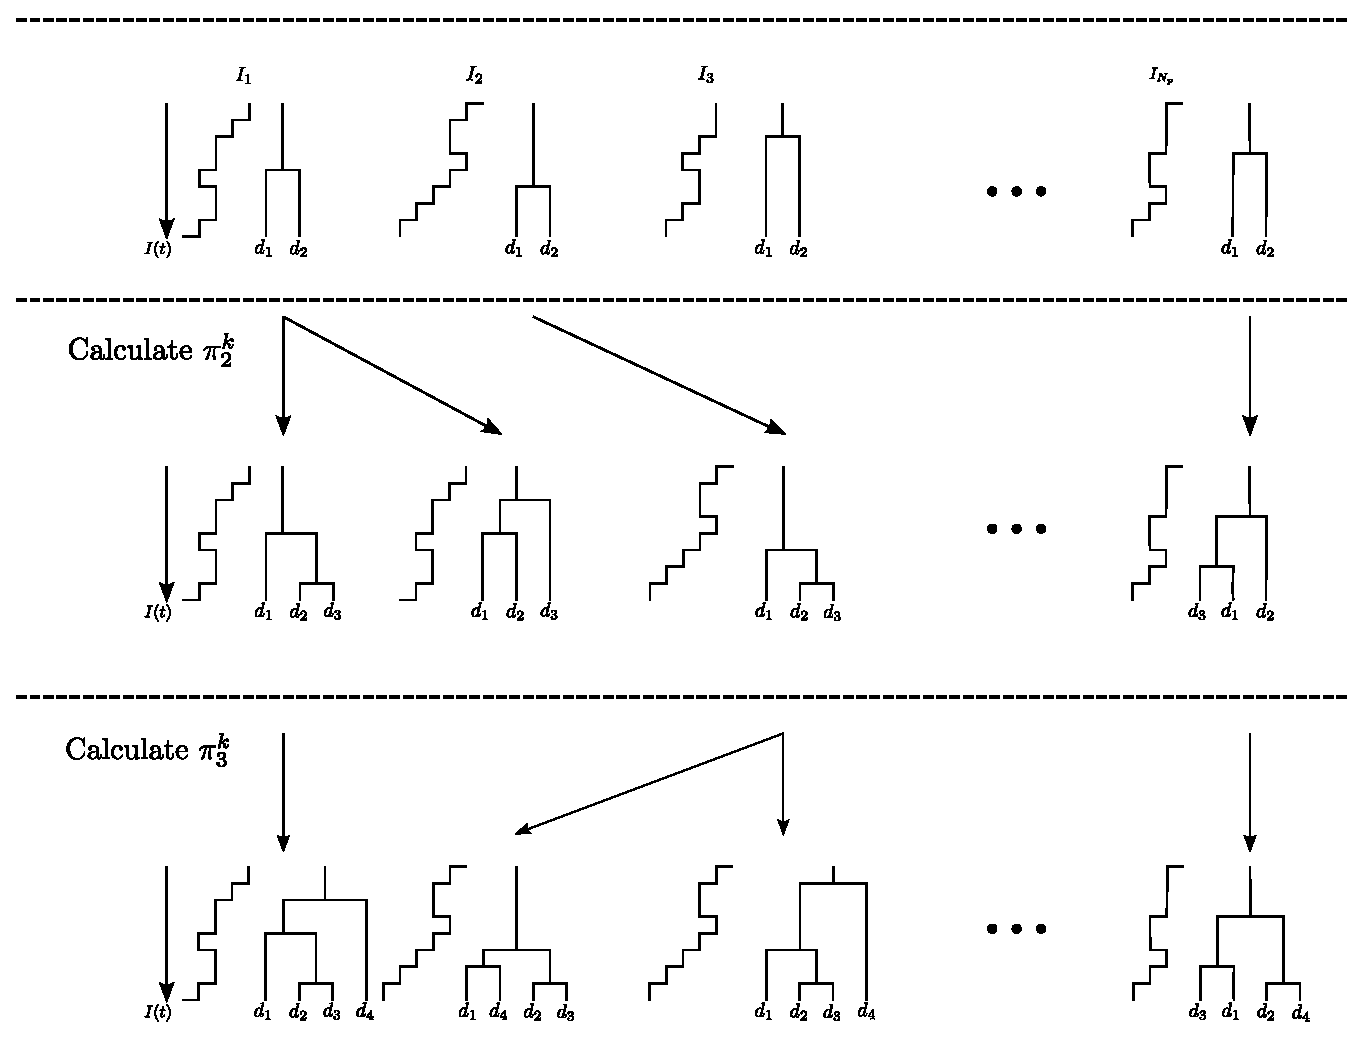
\includegraphics[width=0.8\textwidth]{smc.eps}
\caption{Illustration of particle filter for generating posterior $\{\mathcal{G}, \mathbf{I}\}$ distribution for $3$ sequences\label{fig:smc}}
\end{figure}


\subsubsection{Initialisation}
We draw $N_p$ trajectories of the infected population size given the current parameters by sampling $\{\mathbf{I}^1,..., \mathbf{I}^{N_p}\}$ from $p(\mathbf{I} \mid \Theta_{I})$. We construct trees with $2$ tips for each of $\{\mathbf{I}^1,..., \mathbf{I}^{N_p}\}$,
by sampling from $p(g_2 \mid \mathbf{I}^i), i=1,...,N_p$, from the process described in Algorithm \ref{alg:g_from_I_g}. We calculate a weight for each of the particles $\{g_2^k,  I^k \mid k=1,..,N_p\}$, $w_2^k = p(d_1, d_2 \mid \mu, g_2^k)$, using the tree likelihood calculated by Felsenstein's pruning algorithm, and $\pi_{2}^k = w_{2}^{k} / \sum_{k'} w_{2}^{k'}$

\subsubsection{Resampling step}
Draw a new particle cloud by resampling the existing one. Denote $p(a_n^k \mid \pi)$ as the discrete distribution on $1,...,N_p$, with probability mass function $\pi$, and sample the indices of existing particles by drawing $a_n^k \sim p(a_n^k \mid \pi), k=1,...,N_p$.  

\subsubsection{Growing each tree}
Sample $g_{n+1}^k \sim p(g_{n+1}^k \mid g_n^{a_n^k})$ using Algorithm \ref{alg:g_from_I_g}, then calculate a weight for each of the new particles: $w_{n+1}^k=p(d_1,...,d_{n+1} \mid \mu, g_{n+1}^k)$, and set $\pi_{n+1}^k = w_{n+1}^{k} / \sum_{k'} w_{n+1}^{k'}$

\subsubsection{Final tree}
We continue resampling the tree population and growing each tree until we have a population of trees with $N_s$ tips, $\{g_{N_s}^k,  I^k \mid k=1,..,N_p\}$, $w_{N_s}^k = p(\mathcal{D} \mid \mu, g_{N_s}^k)$. The estimate of the likelihood is given by:
$\frac{1}{N_p} \sum_k w_{N_s}^k$



\begin{algorithm}
\caption{Reconstructing ancestral tree $g_{n+1}$ from infected population trajectories $I[t]$, $\mathbf{T}$, given current tree $g_n$. \label{alg:g_from_I_g}}
\begin{algorithmic}
\STATE ${\textrm{Nodes}_{\textrm{anc}}^{n+1}=\{\}}$ , ${\textrm{t}_{\textrm{anc}^{n+1}}=\{\}}$ \COMMENT{list of new ancestral nodes and times, for each host}
\STATE ${\textrm{Nodes}_{\textrm{anc}}^{n}=\{\}}$ , ${\textrm{t}_{\textrm{anc}^{n}}=\{\}}$ \COMMENT{list of old ancestral nodes and times, for each host}
\STATE ${\textrm{Nodes}_{\textrm{ex}}}=\{I[T][1] - P_1, ..., I[T][N_H] - P_{N_H}\}$,   \COMMENT{vector of number of extinct nodes for each host}
\STATE $g_{n+1}=\{\}$ \COMMENT{ancestral tree for sequences $d_1,...,d_{n+1}$}
\STATE $g_{n}$ \COMMENT{ancestral tree for sequences $d_1,...,d_{n}$}
\STATE $M_n$ \COMMENT{record of ancestral nodes that migrate between hosts in constructing $g_n$}
\STATE $n_{\textrm{int}}= N_s + 1$ \COMMENT{internal node of tree}
\STATE Label first $n$ sequences in $\mathcal{D}$ for each host: $\mathcal{L}_1=\{1,...,P_1\}$,  $\mathcal{L}_2=\{P_1+1,...,P_1 + P_2\}$, 
\FOR{$t=T$ \TO $t=1$ \COMMENT{for each event time}}
{
\IF{$t=s_i$, where $i \in 1,...,N_H$ \COMMENT{if at sampling time for host i}}	
{
	\STATE $\textrm{Nodes}_{\textrm{anc}}[i] \gets \mathcal{L}_i $
	\STATE $\textrm{t}_{\textrm{anc}}[i] \gets \{t, t, ..., t\}$
	\STATE Update ${\textrm{Nodes}_{\textrm{anc}}^{n+1}[i+1]}$ , ${\textrm{t}_{\textrm{anc}^{n+1}[i]}}$ if new tip added here.
}
\ENDIF
\IF{event at $t$ = recovery in host $i$}	
	\STATE $\textrm{Nodes}_{\textrm{ex}}[i] \gets \textrm{Nodes}_{\textrm{ex}}[i]  + 1 $
\ENDIF
\IF{event at $t$ = infection within host $i$}	
{
	\STATE Pick a pair of nodes $n_a$, $n_b$ from all nodes (extinct and ancestral) in $i$
	\IF  {$n_a$ and $n_b$ are from $\textrm{Nodes}_{\textrm{anc}}^n[i]$ and  $\textrm{Nodes}_{\textrm{anc}}^{n+1}[i]$} 
	{
		\STATE {\it Coalescent event in host $i$}
		\STATE  Add new edges $\{n_{\textrm{int}}, n_a \}$, $\{n_{\textrm{int}}, n_b \}$ , with lengths $\textrm{t}_{\textrm{anc}}[i][n_a] - t$, $\textrm{t}_{\textrm{anc}}[i][n_b] - t$ to $g^n$:
		\STATE \textbf{break}
	}
	\ELSE
	{
		\STATE $\textrm{Nodes}_{\textrm{ex}}[i] \gets \textrm{Nodes}_{\textrm{ex}}[i]  - 1 $
	}
	\ENDIF
}
\ENDIF
\IF{event at $t$ = transmission of $k$ nodes from host $i$ to host $j$}	
{
	\STATE Pick $k$ nodes $n_a^1,...,n_a^k$ from all nodes (extinct and ancestral) in $i$
	\STATE Pick $k$ nodes $n_b^1,...,n_b^k$ from all nodes (extinct and ancestral) in $j$
	\STATE Move  $n_b^1,...,n_b^k$ to $\textrm{Nodes}_{\textrm{anc}}[i]$ 
	\FOR {$n=1$ \TO $n=k$}
	{
	\IF  {$n_a^n$ is from $\textrm{Nodes}_{\textrm{anc}}[i]$ and $n_b^n$ was from $\textrm{Nodes}_{\textrm{anc}}[j]$} 
	{
		\STATE {\it Coalescent event between host $i$ and host $j$}
		\STATE  Add new edges $\{n_{\textrm{int}}, n_a \}$, $\{n_{\textrm{int}}, n_b \}$ , with lengths $\textrm{t}_{\textrm{anc}}[i][n_a] - t$, $\textrm{t}_{\textrm{anc}}[i][n_b] - t$ to $g$
		\STATE Replace $n_a$ and $n_b$ in $\textrm{Nodes}_{\textrm{anc}}[i]$ with internal node $n_{\textrm{int}}$ with corresponding time $t$
		\STATE $n_{\textrm{int}} \gets n_{\textrm{int}} + 1$
	}
	\ELSE
	{
		\IF {$n_b^n$ was from $\textrm{Nodes}_{\textrm{anc}}[j]$}
		{
		\STATE $\textrm{Nodes}_{\textrm{ex}}[i] \gets \textrm{Nodes}_{\textrm{ex}}[i]  - 1 $
		}
		\ELSE
		{
		\STATE $\textrm{Nodes}_{\textrm{ex}}[j] \gets \textrm{Nodes}_{\textrm{ex}}[j]  - 1 $
		}
		\ENDIF
	}
	\ENDIF
	}
	\ENDFOR
}
\ENDIF

}
\ENDFOR
\end{algorithmic}
\end{algorithm}
\section{Model output}
This section illustrates the output from the model for different sets of parameters. 
\subsection{Population history}
See Figures \ref{fig:poptraj1} and \ref{fig:poptraj2}. Each subplot shows the infected population size against time for $5$ hosts $I_1(t),...,I_5(t)$. The time that each host is sampled is shown in red, with a marker to show the number of sequences that was sampled. This shows that the trajectories are valid, since the infected population sizes at time of sampling is greater than the number of sequences. The black arrows between the plots show the times of transmission events between the hosts.
\subsubsection{Figure \ref{fig:poptraj1}}
\begin{eqnarray}
\beta&=& 
\left(
\begin{array}{ccccc}
 4  &	 0.0004 & 0.0004 & 0  & 0\\
 0 & 4  & 0   & 0.0004  & 0\\
 0 &  0  &   4 & 0 & 0.0004\\
 0 &  0 & 0  &4 & 0\\
 0 & 0  &  0 & 0 & 4
 \end{array}
\right)\nonumber\\
\gamma&=&0.2\nonumber\\
t_{off} &=& 7\nonumber\\
\theta_K &=& 0.01
\end{eqnarray}
\subsubsection{Figure \ref{fig:poptraj2}}
\begin{eqnarray}
\beta&=& 
\left(
\begin{array}{ccccc}
 2  &	 0.004 & 0.004 & 0  & 0\\
 0 & 2  & 0   & 0.004  & 0\\
 0 &  0  &   2 & 0 & 0.004\\
 0 &  0 & 0  &2 & 0\\
 0 & 0  &  0 & 0 & 2
 \end{array}
\right)\nonumber\\
\gamma&=&0.4\nonumber\\
t_{off} &=& 7\nonumber\\
\theta_K &=& 0.01
\end{eqnarray}

\begin{figure}[h]
\centering
\subfigure[]{
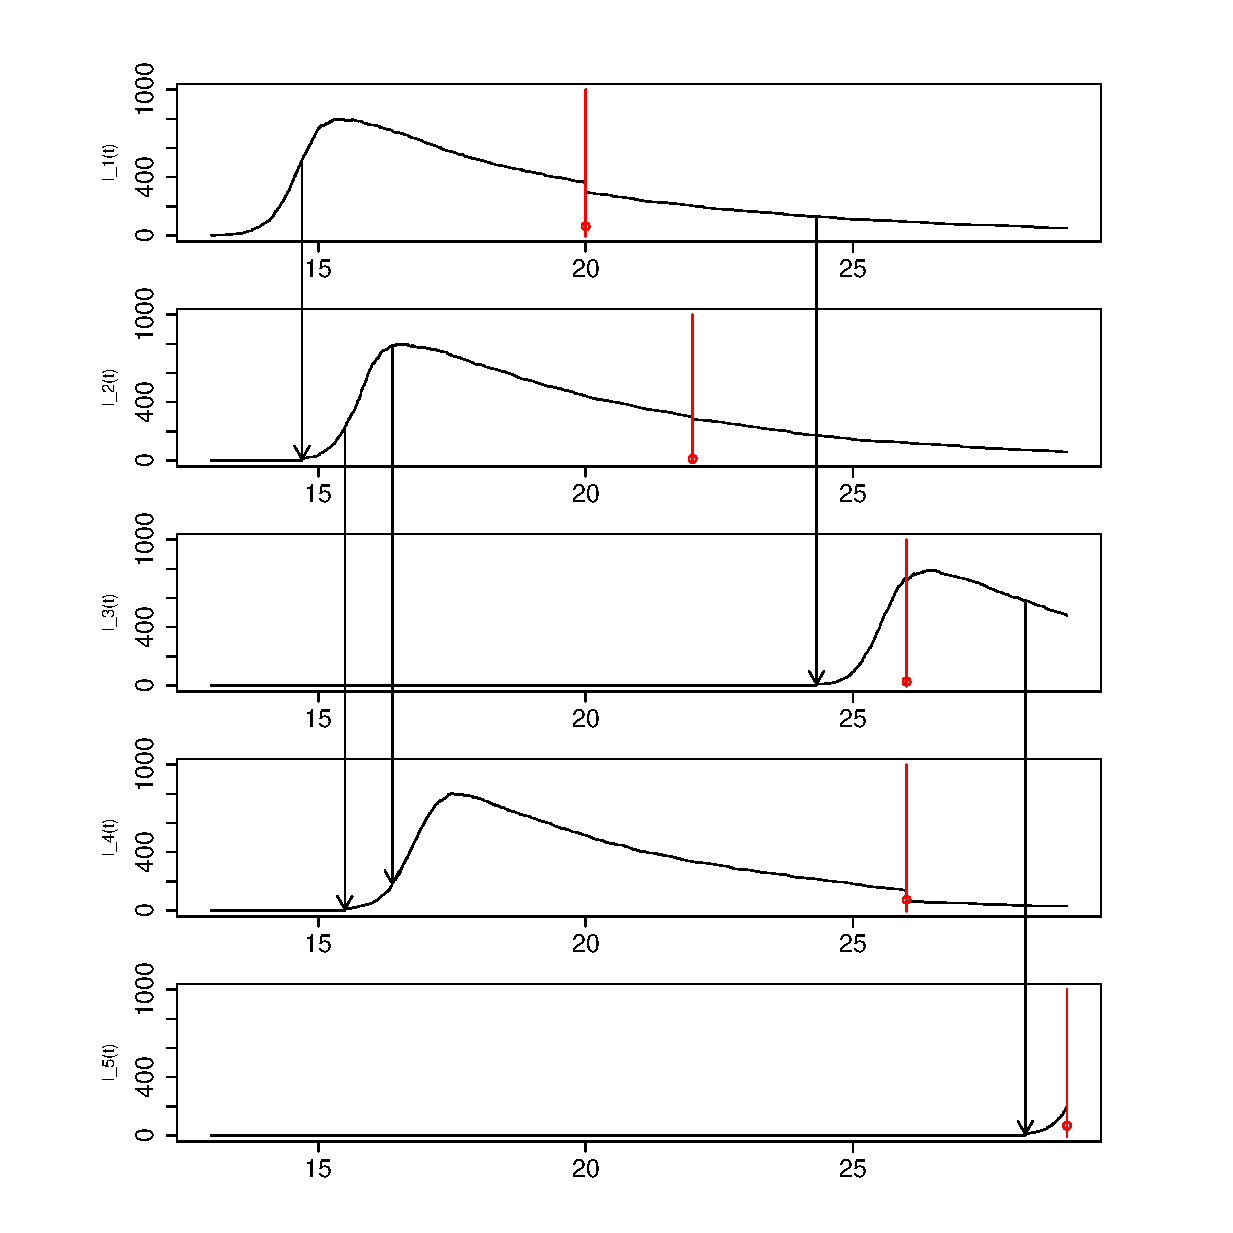
\includegraphics[width=0.42\textwidth]{poptraj001.eps}
\label{fig:poptraj1}
}
\subfigure[]{
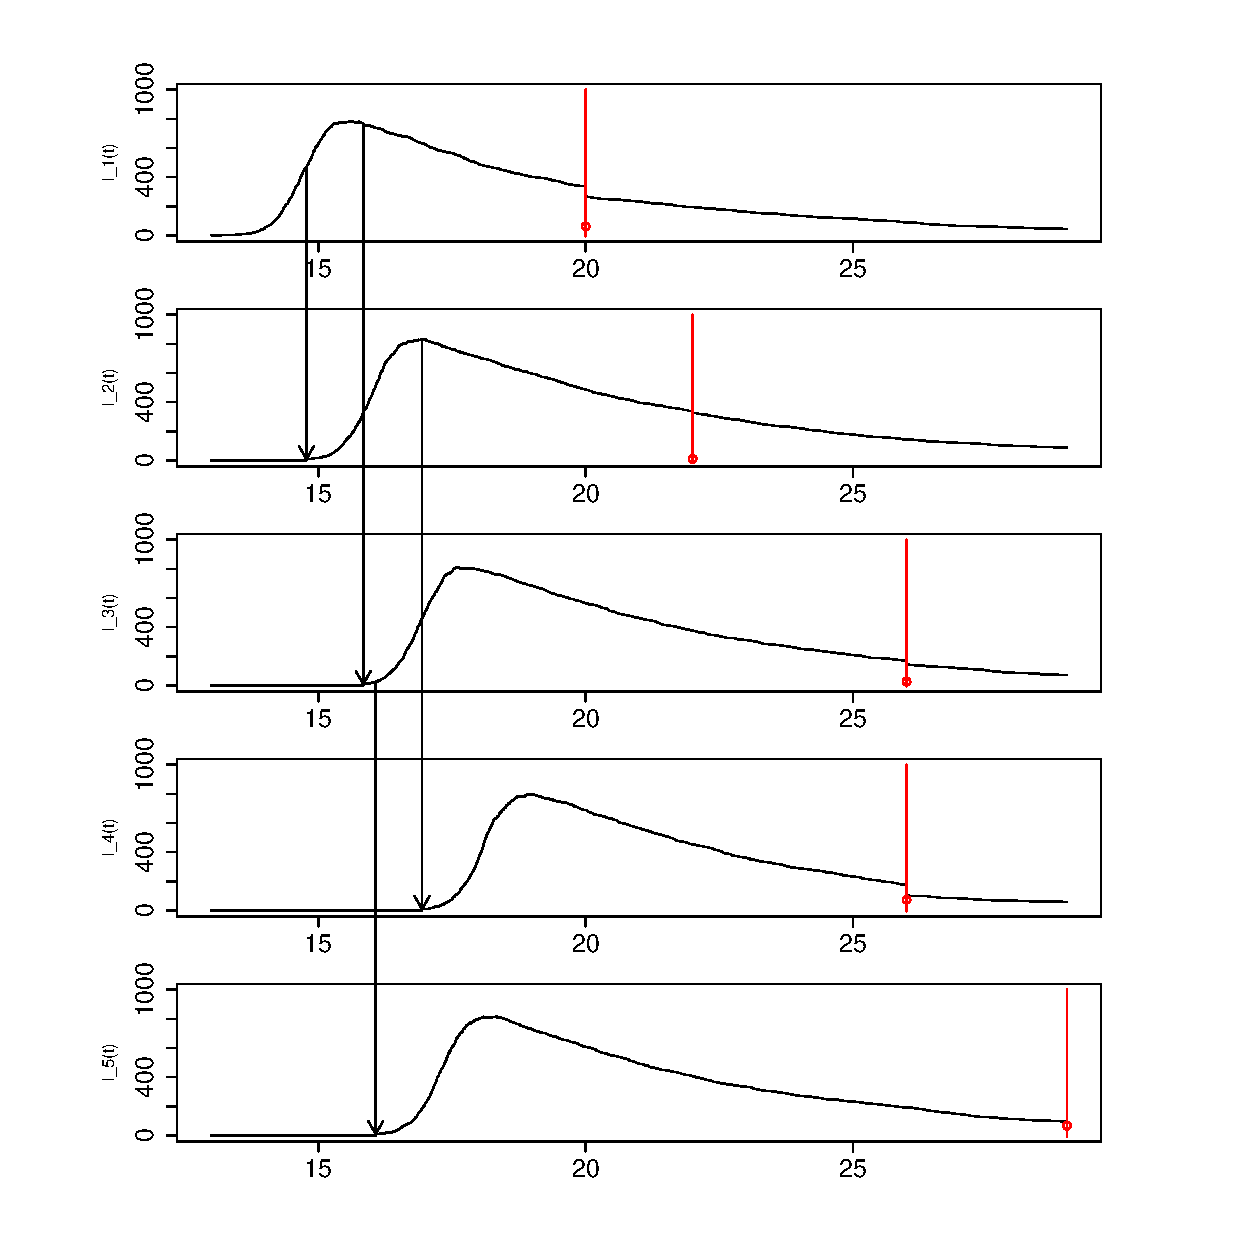
\includegraphics[width=0.42\textwidth]{poptraj002.eps}
\label{fig:poptraj2}
}\\
\subfigure[]{
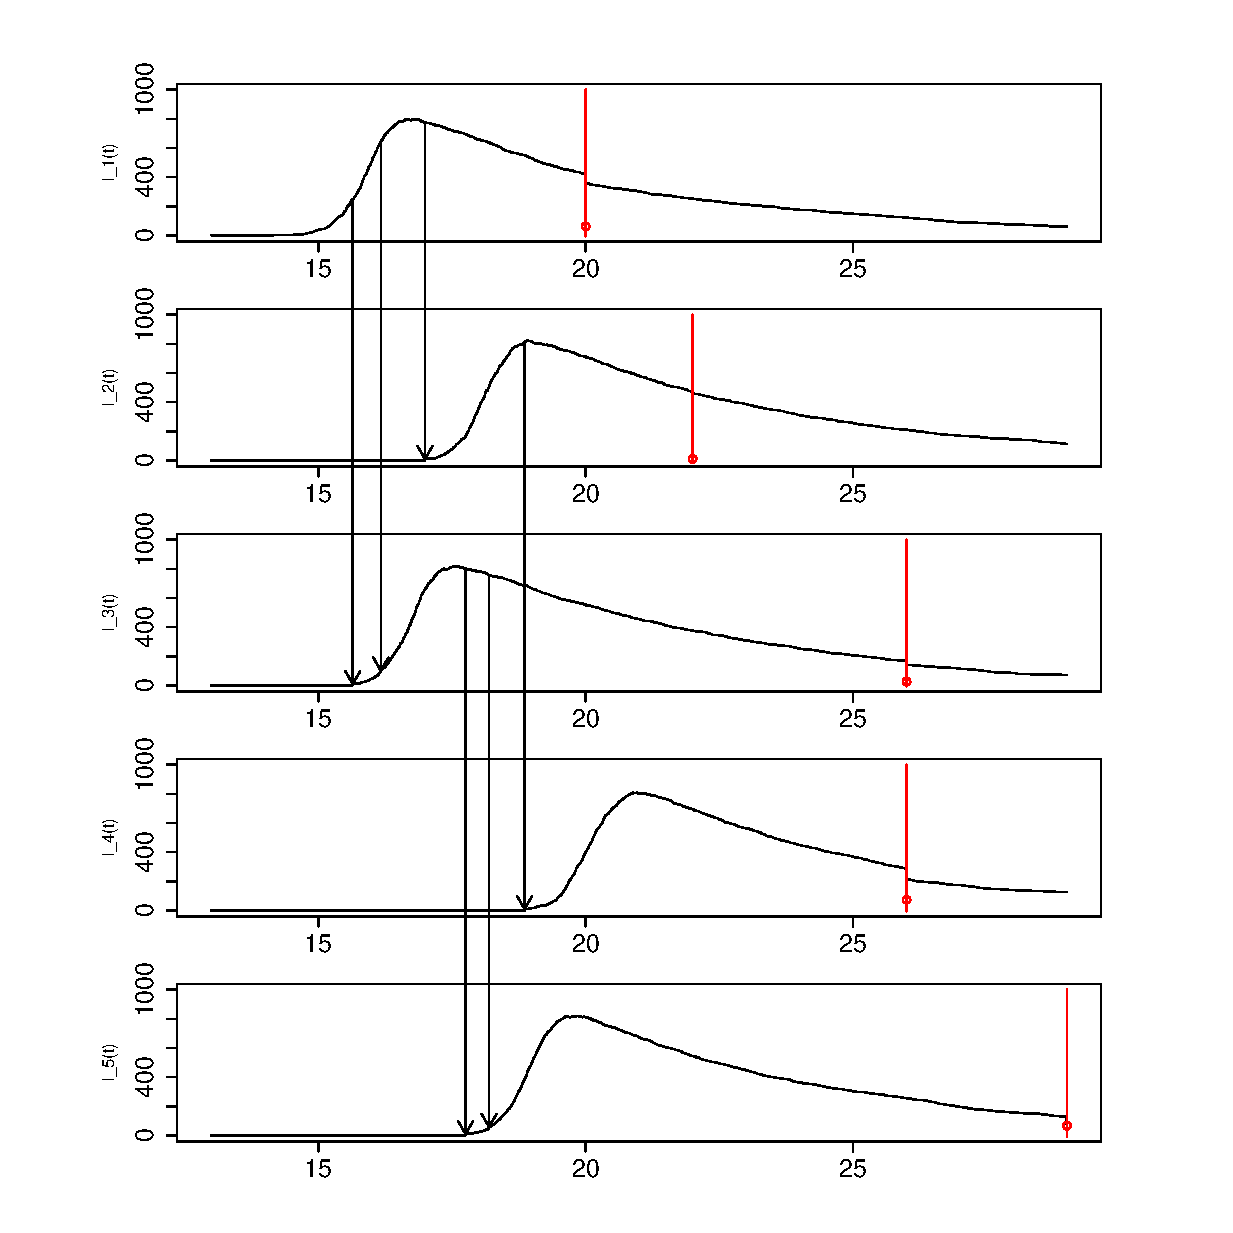
\includegraphics[width=0.42\textwidth]{poptraj003.eps}
\label{fig:poptraj3}
}
\subfigure[]{
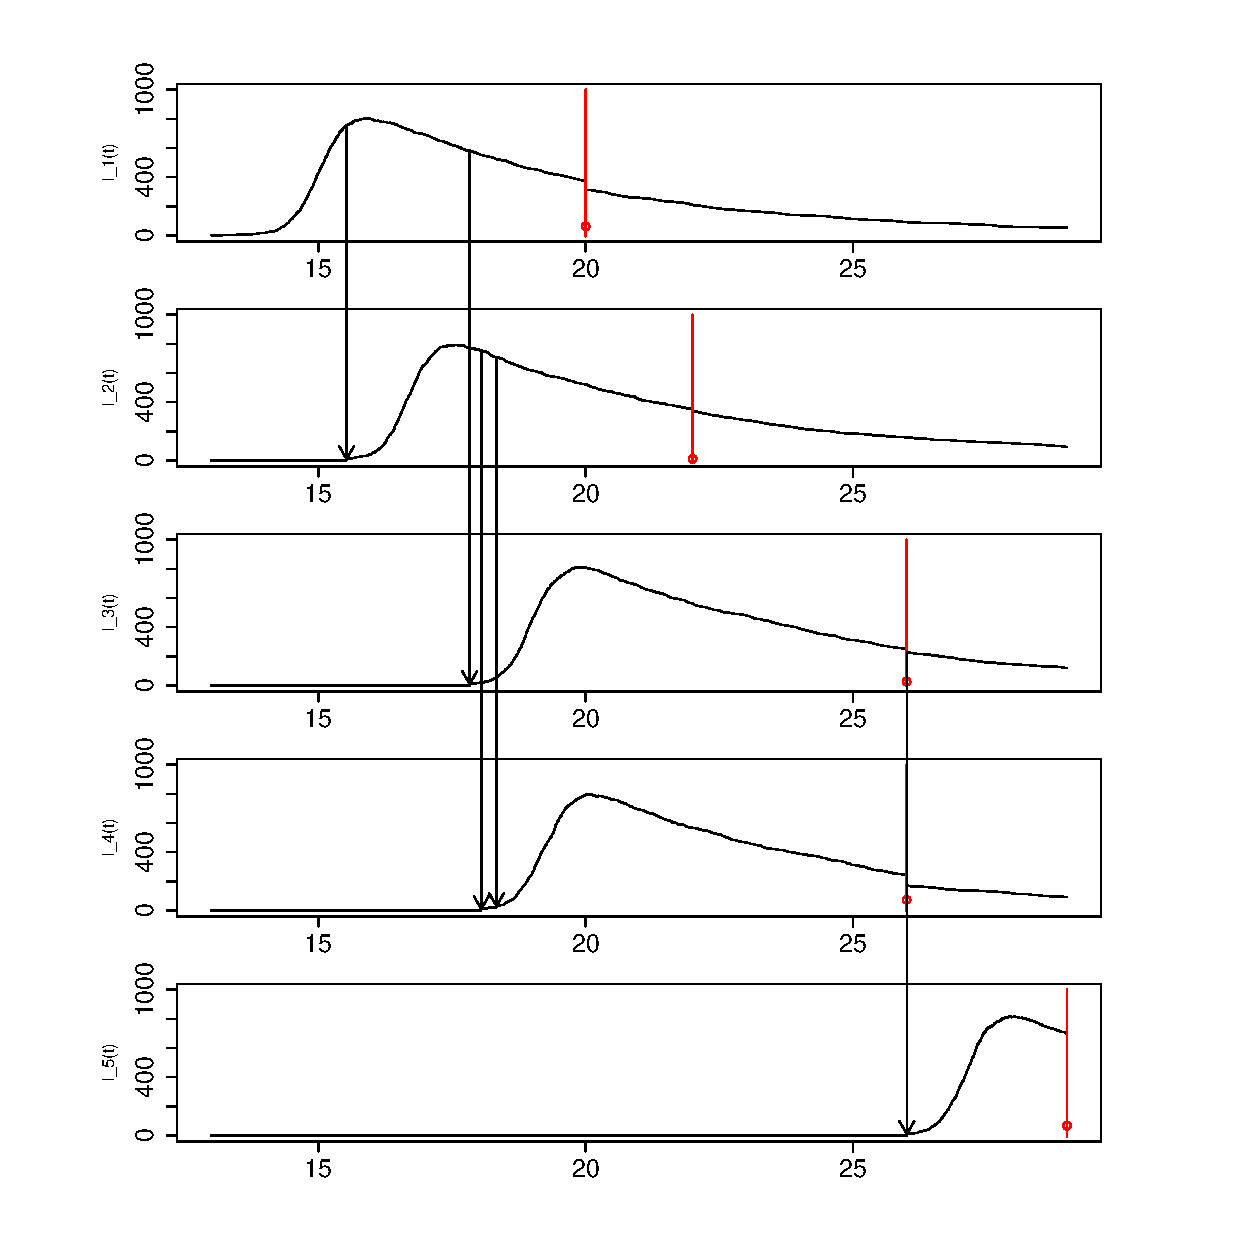
\includegraphics[width=0.42\textwidth]{poptraj004.eps}
\label{fig:poptraj4}
}\\
\subfigure[]{
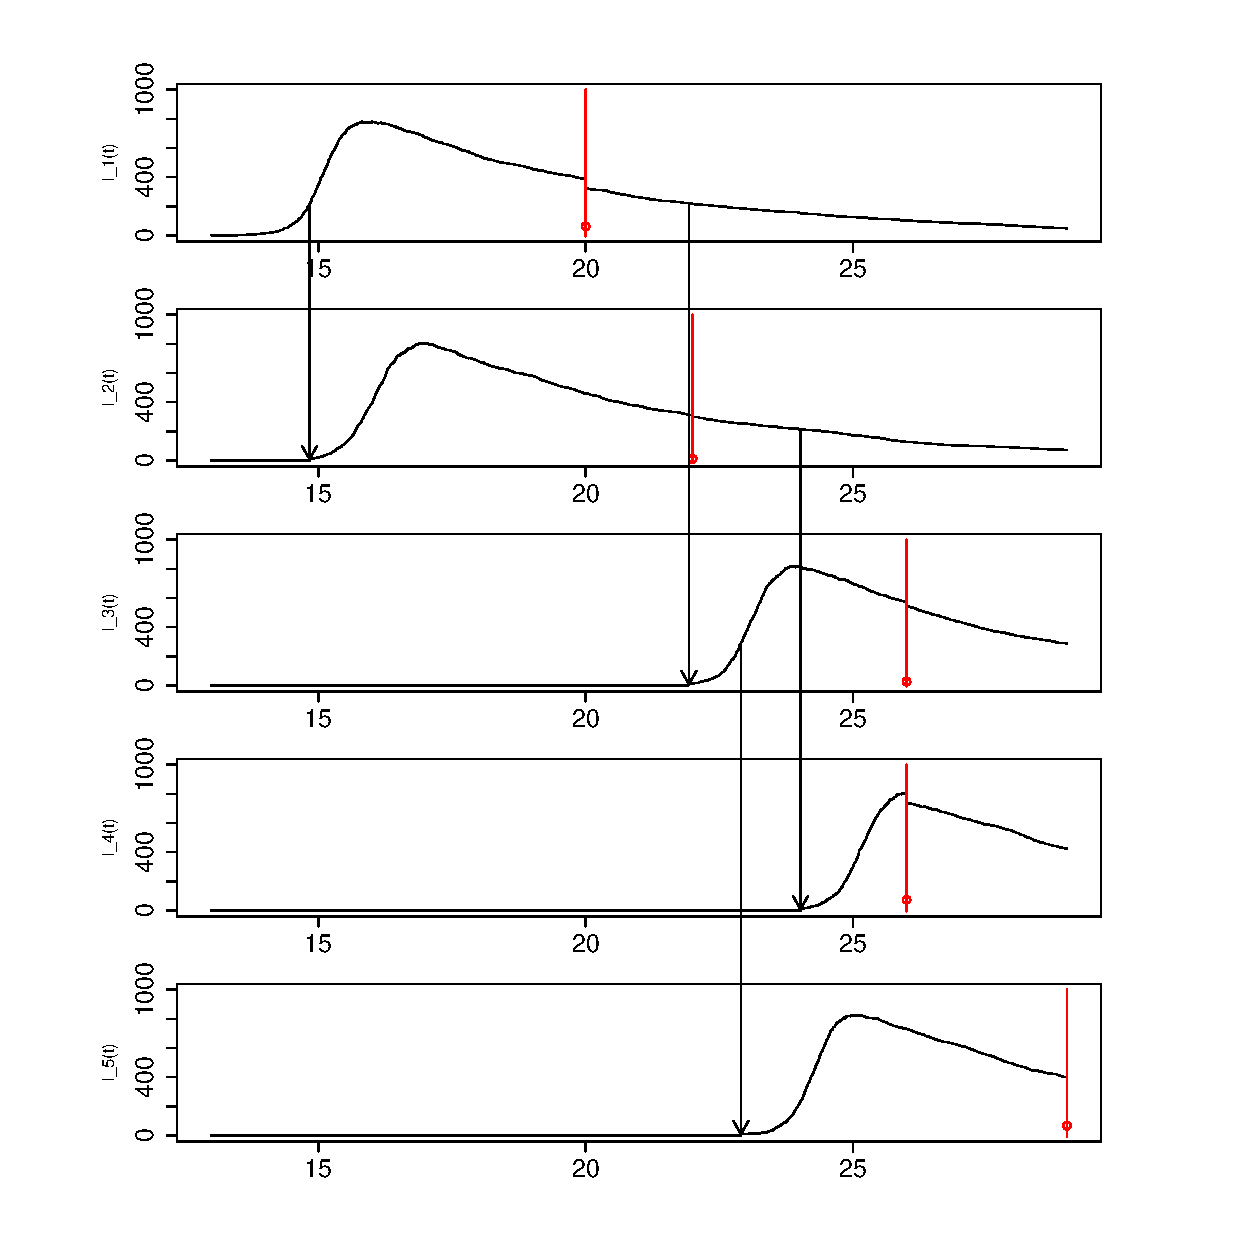
\includegraphics[width=0.42\textwidth]{poptraj005.eps}
\label{fig:poptraj5}
}
\subfigure[]{
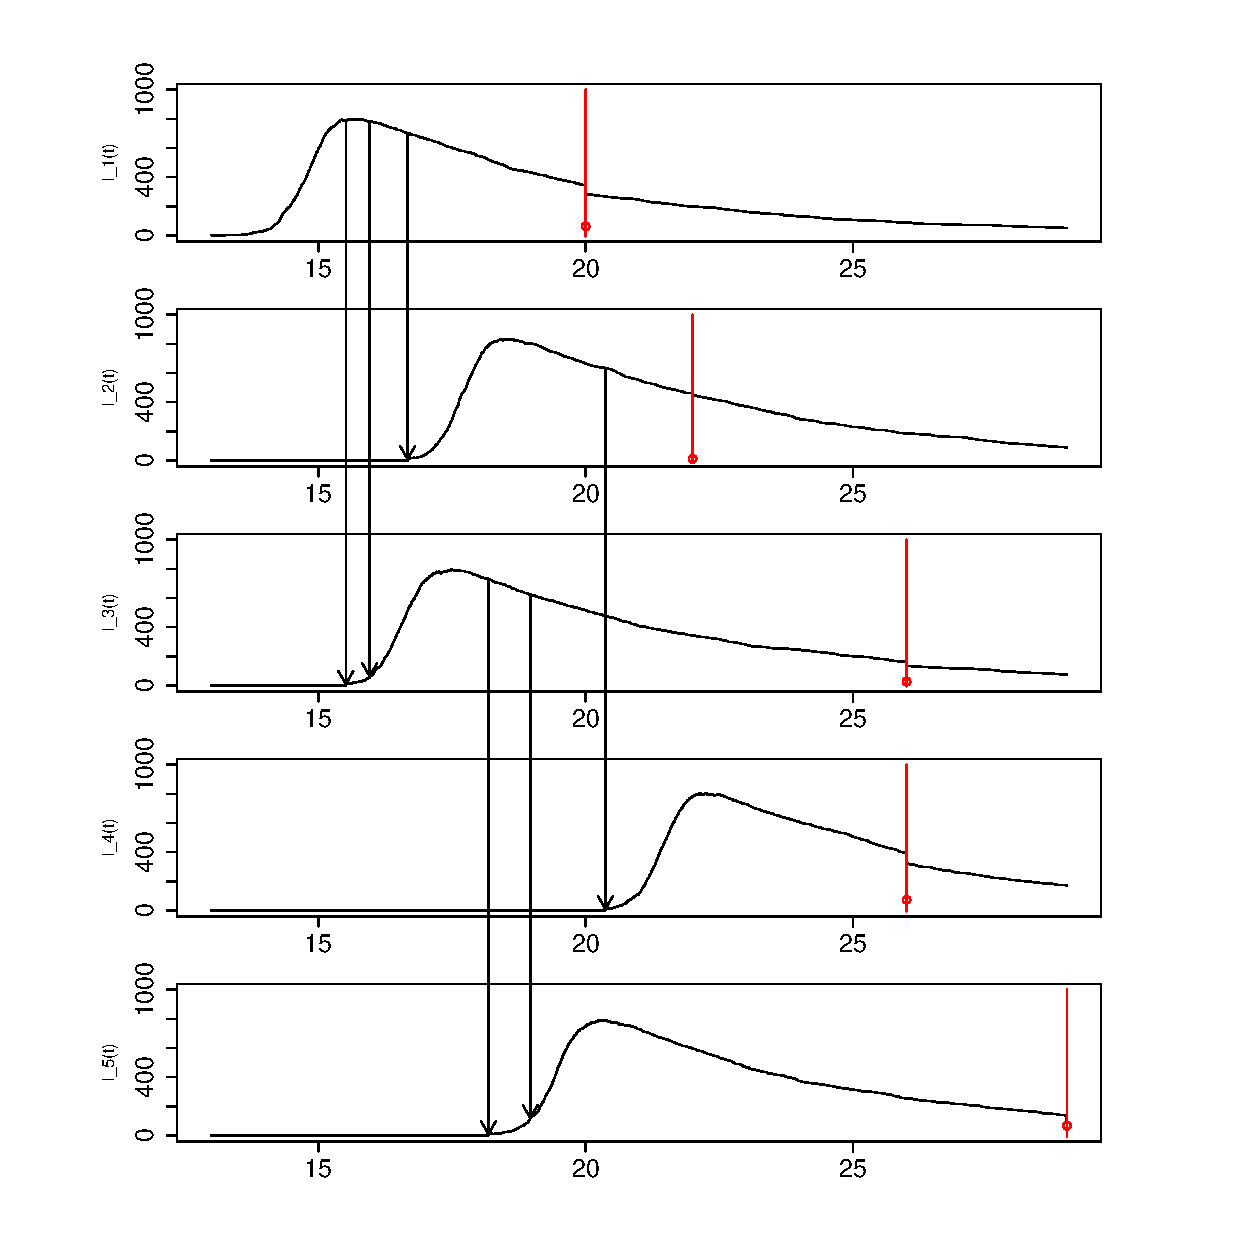
\includegraphics[width=0.42\textwidth]{poptraj006.eps}
\label{fig:poptraj6}
}
\caption{$6$ infected population trajectories for model}
\label{fig:poptraj1}
\end{figure}


\begin{figure}[h]
\centering
\subfigure[]{
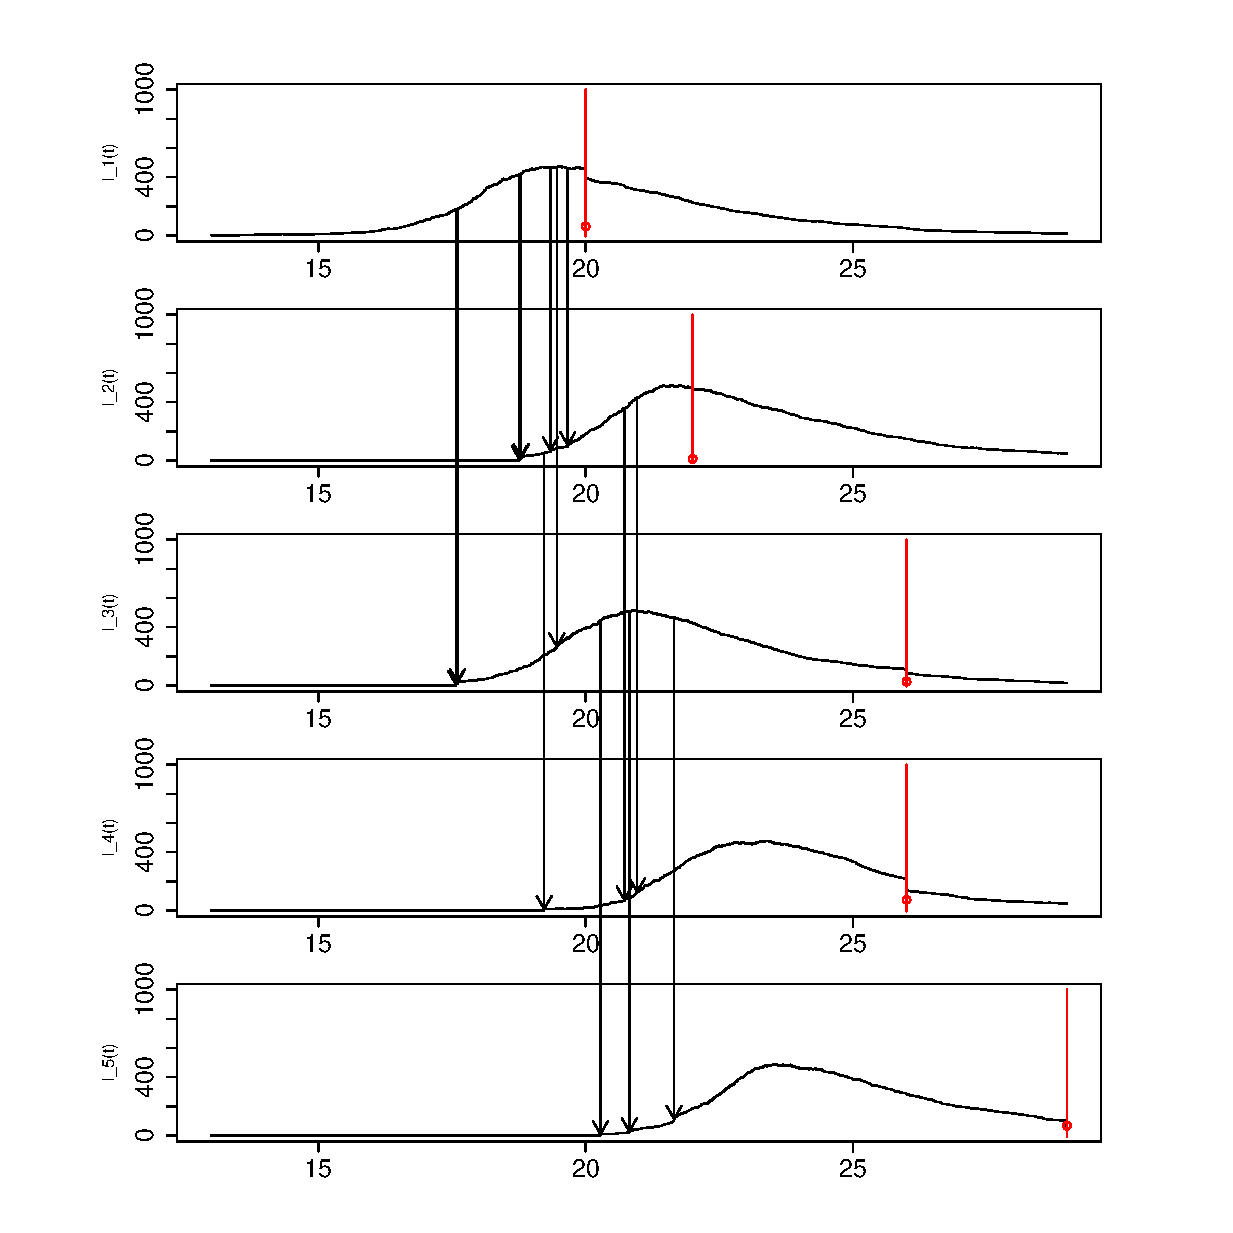
\includegraphics[width=0.42\textwidth]{poptraj007.eps}
\label{fig:poptraj7}
}
\subfigure[]{
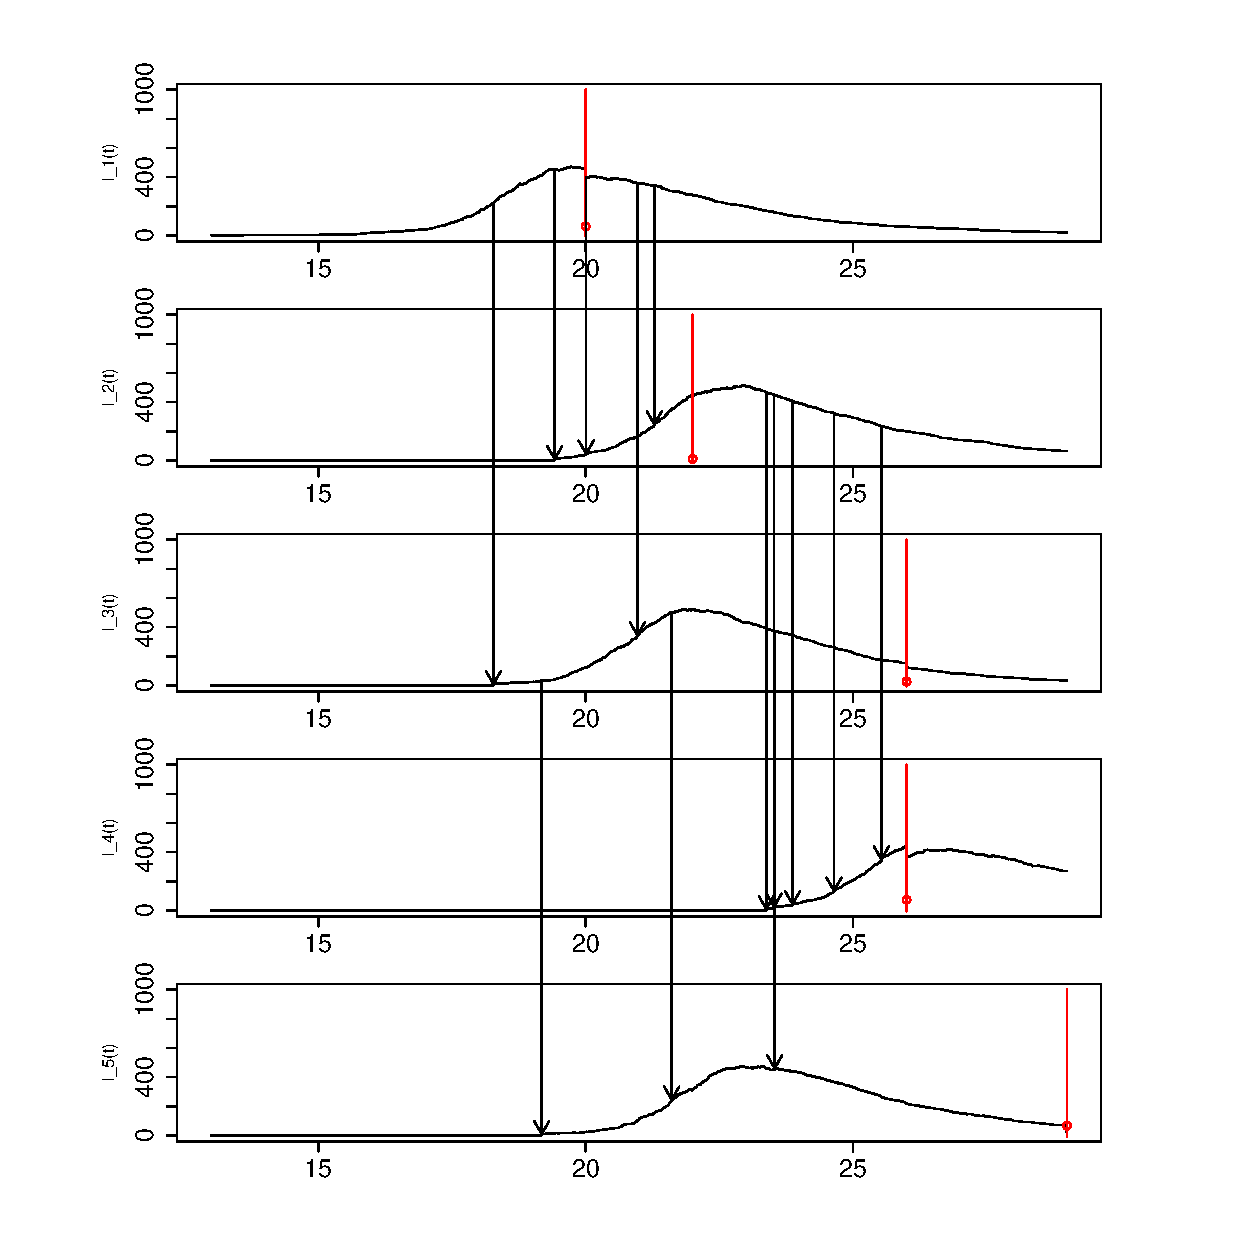
\includegraphics[width=0.42\textwidth]{poptraj008.eps}
\label{fig:poptraj8}
}\\
\subfigure[]{
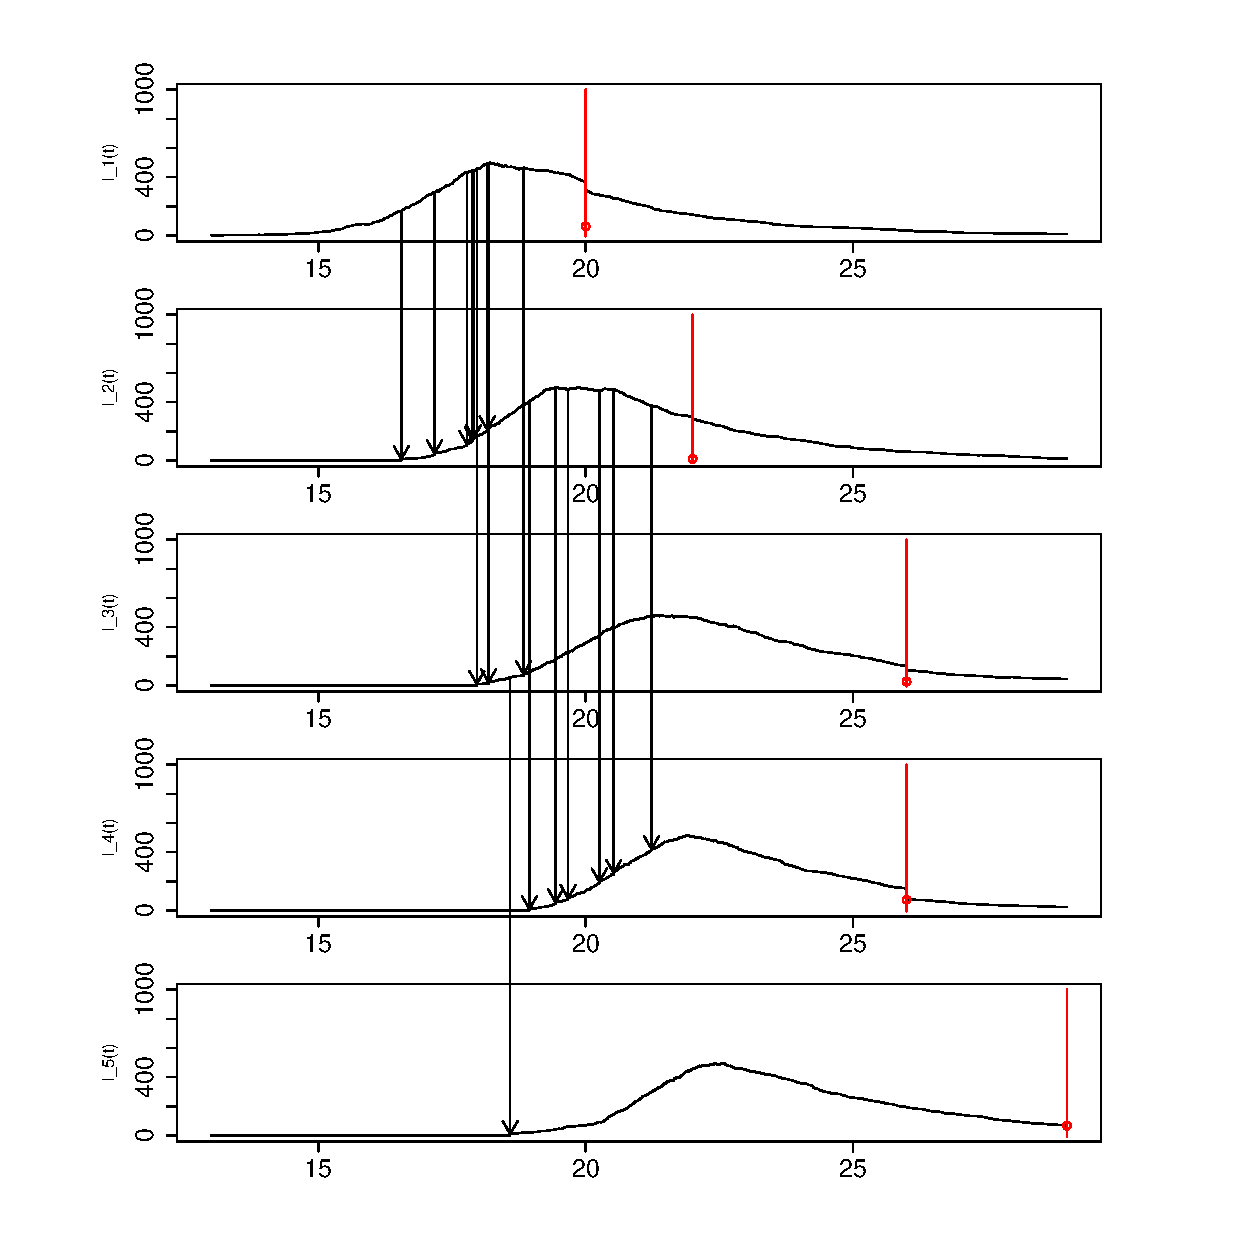
\includegraphics[width=0.42\textwidth]{poptraj009.eps}
\label{fig:poptraj9}
}
\subfigure[]{
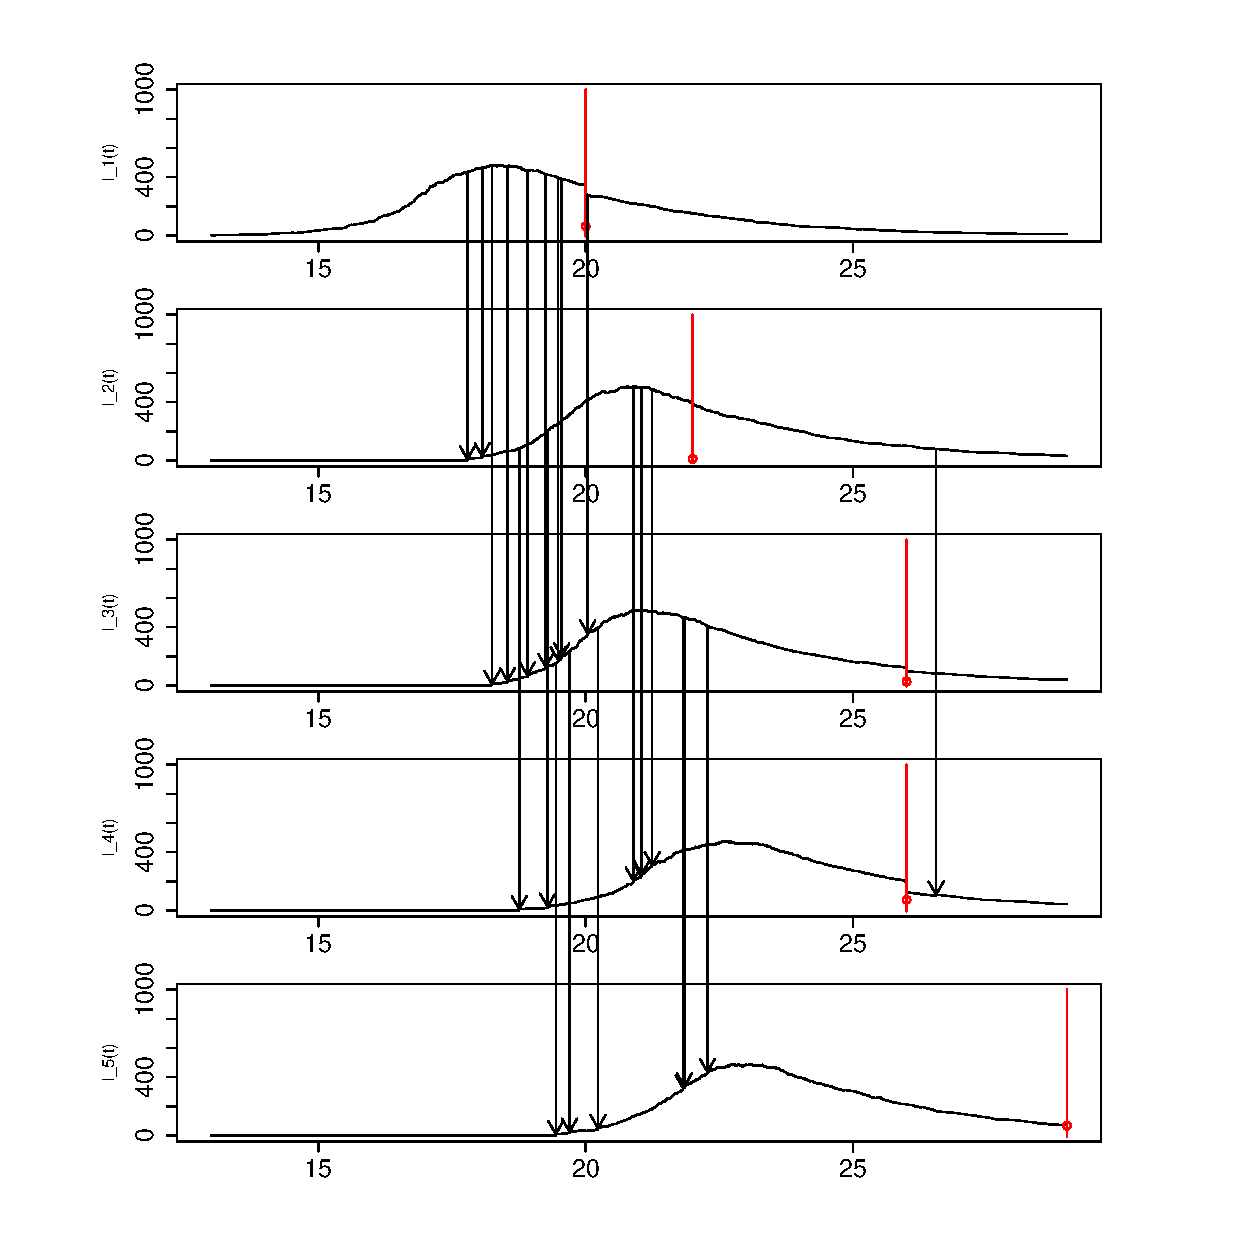
\includegraphics[width=0.42\textwidth]{poptraj010.eps}
\label{fig:poptraj10}
}\\
\subfigure[]{
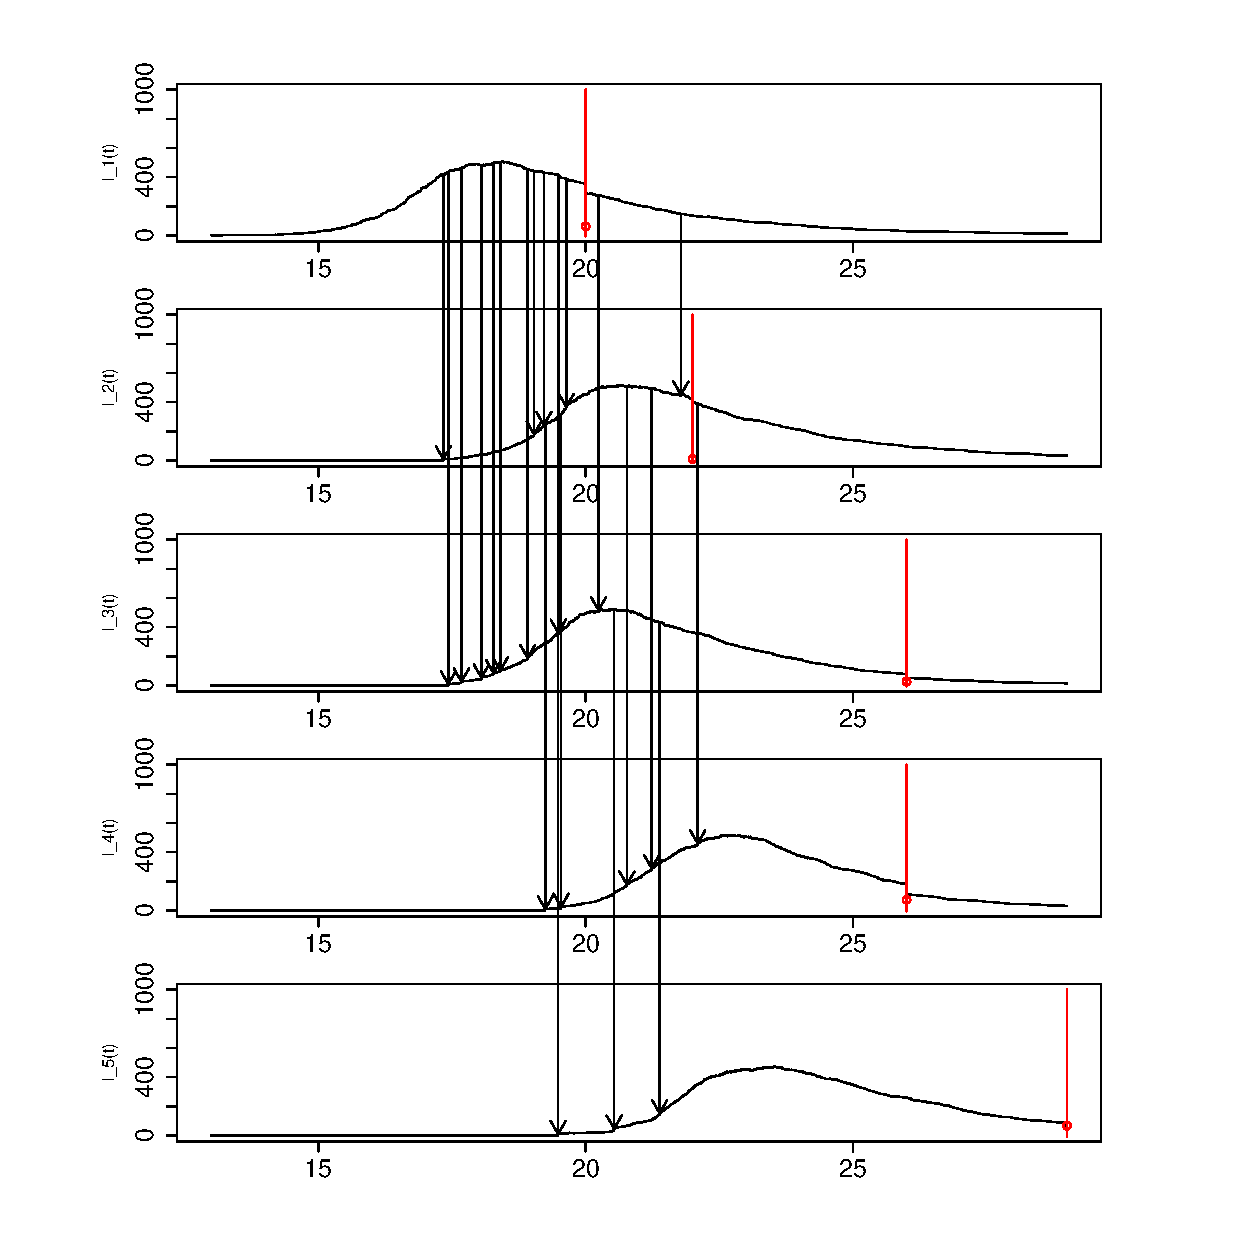
\includegraphics[width=0.42\textwidth]{poptraj011.eps}
\label{fig:poptraj11}
}
\subfigure[]{
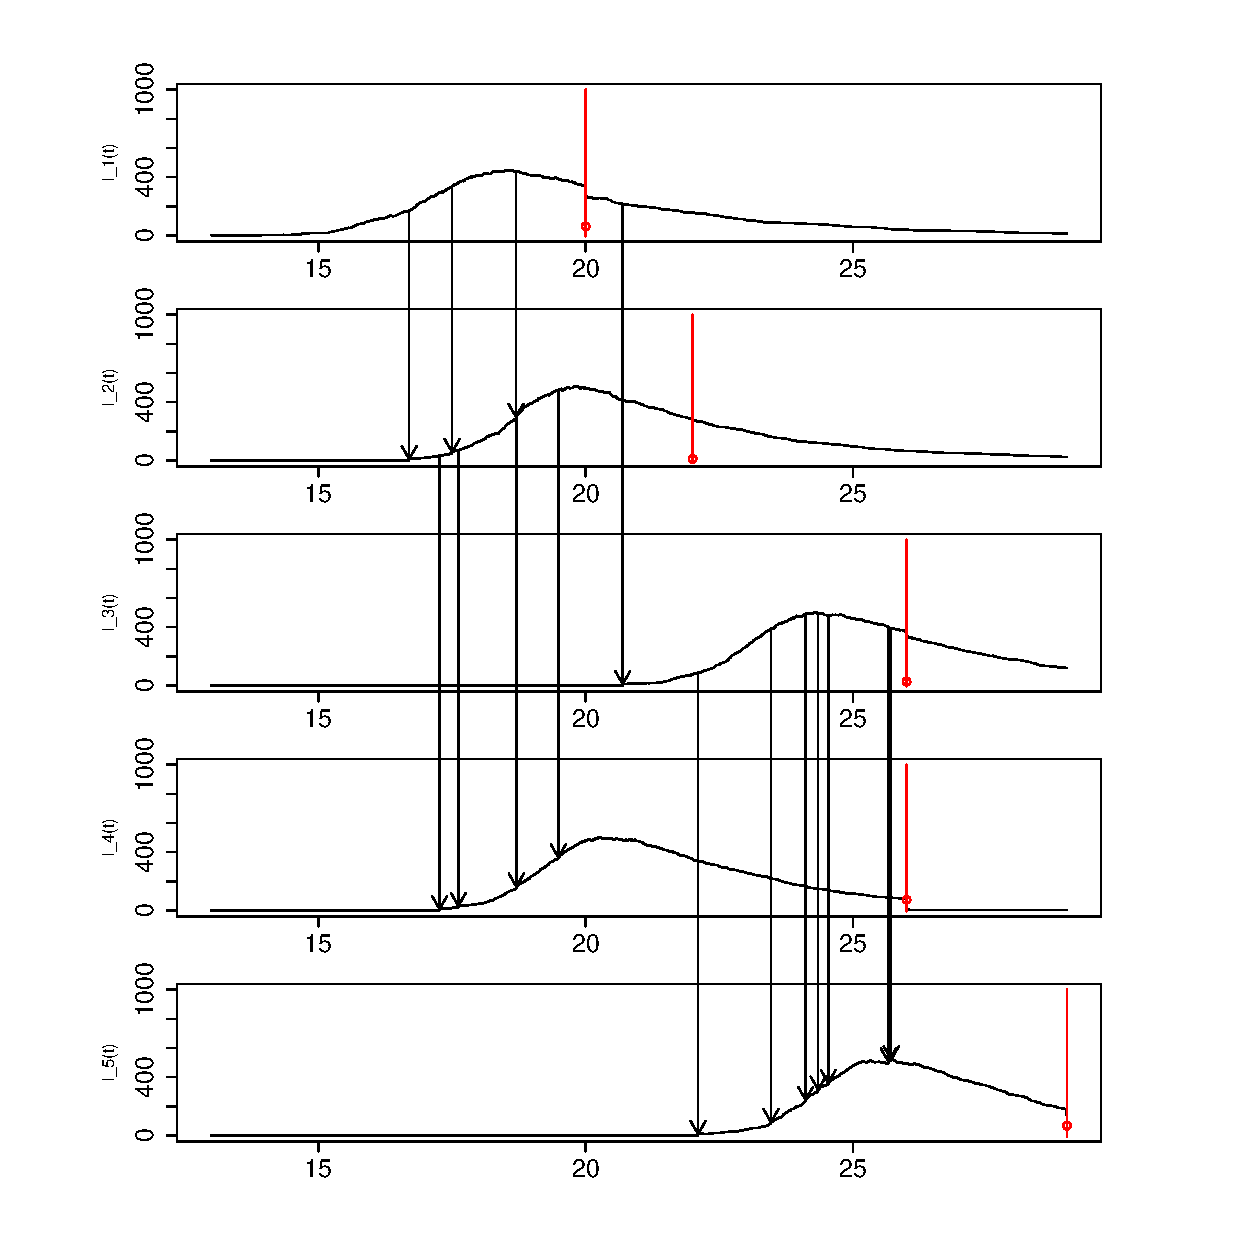
\includegraphics[width=0.42\textwidth]{poptraj012.eps}
\label{fig:poptraj12}
}
\caption{$6$ infected population trajectories for model}
\label{fig:poptraj2}
\end{figure}


\section{Summary}
\begin{tabular}{|l|l|}
\hline 
\multicolumn{2}{|c|}{Data}\\
\hline
Number of hosts & $N_h$  \\
Number of sequences in hosts & $P_1,...,P_{N_h}$ \\
Sequences & $\mathcal{D}=\{\mathbf{d}_{1,1},...,\mathbf{d}_{1,P_1}\},...,\{\mathbf{d}_{N_h,1},...,\mathbf{g}_{1,P_{N_h}}\} $ \\
Time of sequences/ host sampling& $\mathbf{S}=\{s_1,...,s_{N_h}\}$ \\
Number of yards & $N_y$  \\
Fraction of yard infected & $\alpha_1,...,\alpha_{N_y}$ \\
\hline 
\multicolumn{2}{|c|}{SIR model parameters}\\
\hline
Infection rates for particles from  & $\beta_{i,j}, i \in 1,...,N_h, j \in 1,...,N_h$ \\
host $i$ and host $j$ & \\
Recovery rate for particles in host $i$ & $\gamma$ \\
Initial number of susceptible particles in each host & $N$ \\
\hline 
\multicolumn{2}{|c|}{SIR model output}\\
\hline
SIR population trajectories & $S(t), I(t), R(t)$ \\
Summary of infection/ recovery events and times & $\mathbf{T}$, $\mathbf{T}_i=\{\textrm{time of event, from, to, event type} \}$ \\
Summary of infection events & $\mathbf{T}^R$, $\mathbf{T}^R_i=\{b_i, H_p,H_{c_1}, H_{c_2}] \}$ \\
from reconstructed tree & \\
\hline 
\multicolumn{2}{|c|}{Genealogy $\mathcal{G}$}\\
\hline
Number of tips & should be $\sum_i^{N_h}P_i$ \\
Bifurcation/'significant' infection times & $b_1,...,b_{\sum_i^{N_h}P_i}$ \\
derived from SIR model&  \\
Topology & $\mathcal{T} $\\
\hline
\multicolumn{2}{|c|}{Mutation model}\\
\hline
Mutation rate & $\mu$ \\
Other parameters & relative rate matrix, genealogy $\mathcal{G}$ \\
\hline
\end{tabular}
\bibliography{phylodynamic}
\bibliographystyle{plain}
\end{document}
